\documentclass{article} % For LaTeX2e
\usepackage{iclr2027_conference,times}

% Optional math commands from https://github.com/goodfeli/dlbook_notation.
\input{math_commands.tex}

\usepackage{hyperref}
\usepackage{url}
\usepackage{booktabs}
\usepackage{xspace}
\usepackage{amsmath}
\usepackage{amssymb}
\usepackage{mathtools}
\usepackage{amsthm}

\newtheorem{theorem}{Theorem}
\theoremstyle{definition}
\newtheorem{definition}[theorem]{Definition}


% Listings for PDDL domains
\usepackage{listings}
\usepackage{caption}

\definecolor{pddlKeyword}{RGB}{0, 0, 130}
\definecolor{pddlLogic}{RGB}{90, 40, 90}
\definecolor{pddlVariable}{RGB}{120, 0, 0}

\lstdefinelanguage{PDDL}{
  morekeywords={
    :action,:parameters,:precondition,:effect,
    :domain,:requirements,:types,:predicates,:objects
  },
  morekeywords=[2]{and,not},
  sensitive=true,
  morecomment=[l]{;},
  morestring=[b]",
  alsoletter={:,-,?}, % treat :, -, ? as part of "words"
  keywordstyle=[1]\color{pddlKeyword}\bfseries,
  keywordstyle=[2]\color{pddlLogic}\bfseries, % ← different color for and/not
  stringstyle=\color{orange},
    literate=
    {?x}{{\color{pddlVariable}?x}}2
    {?y}{{\color{pddlVariable}?y}}2
    {?z}{{\color{pddlVariable}?z}}2
    {?u}{{\color{pddlVariable}?u}}2
}

\lstset{
  language=PDDL,
  basicstyle=\ttfamily\footnotesize,
  keywordstyle=\color{pddlKeyword}\bfseries,
  commentstyle=\color{pddlComment}\itshape,
  stringstyle=\color{orange},
  columns=fullflexible,
  keepspaces=true,
  breaklines=true,
  breakatwhitespace=false,
  xleftmargin=1em,
  framexleftmargin=1em,
  linewidth=\linewidth,
  aboveskip=0.5\baselineskip,
  belowskip=0.5\baselineskip
}


% Extra commands

\newcommand{\bw}{\texttt{blocksworld}\xspace}
\newcommand{\fr}{\texttt{ferry}\xspace}
\newcommand{\np}{\texttt{npuzzle}\xspace}
\newcommand{\mz}{\texttt{maze}\xspace}
\newcommand{\lgt}{\texttt{logistics}\xspace}


\newcommand{\sift}{\textsc{sift}\xspace}
\newcommand{\strips}{\textsc{strips}\xspace}
\newcommand{\brasp}{\textsc{B-RASP}\xspace}

\newcommand{\Omit}[1]{}


\title{Learning Lifted World Models with Transformers}
%\title{Learning Lifted STRIPS Models with Transformers}
% Carlos - I prefer to leave "STRIPS" out of the title

% Authors must not appear in the submitted version. They should be hidden
% as long as the \iclrfinalcopy macro remains commented out below.
% Non-anonymous submissions will be rejected without review.

\author{Antiquus S.~Hippocampus, Natalia Cerebro \& Amelie P. Amygdale \thanks{ Use footnote for providing further information
about author (webpage, alternative address)---\emph{not} for acknowledging
funding agencies.  Funding acknowledgements go at the end of the paper.} \\
Department of Computer Science\\
Cranberry-Lemon University\\
Pittsburgh, PA 15213, USA \\
\texttt{\{hippo,brain,jen\}@cs.cranberry-lemon.edu} \\
\And
Ji Q. Ren \& Yevgeny LeNet \\
Department of Computational Neuroscience \\
University of the Witwatersrand \\
Joburg, South Africa \\
\texttt{\{robot,net\}@wits.ac.za} \\
\AND
Coauthor \\
Affiliation \\
Address \\
\texttt{email}
}

% The \author macro works with any number of authors. There are two commands
% used to separate the names and addresses of multiple authors: \And and \AND.
%
% Using \And between authors leaves it to \LaTeX{} to determine where to break
% the lines. Using \AND forces a linebreak at that point. So, if \LaTeX{}
% puts 3 of 4 authors names on the first line, and the last on the second
% line, try using \AND instead of \And before the third author name.

\newcommand{\fix}{\marginpar{FIX}}
\newcommand{\new}{\marginpar{NEW}}

%\iclrfinalcopy % Uncomment for camera-ready version, but NOT for submission.
\begin{document}


\maketitle

% >> New abstract (Update on OpenReview!)
\begin{abstract}
Recent work has studied whether transformers can learn world models through next-token prediction.
In this paper, we address this question for \textit{lifted models}, i.e., abstract world models that generalize across different numbers of objects.
To this end, we leverage \strips, a logic-based formalism for specifying lifted, interpretable world models.
We propose two transformer architectures for learning \strips models:
the Lifted \strips (LS) Transformer, with built-in symbolic structure and parameters that map directly to \strips;
and the Lifted Stick-Breaking (LB) Transformer, a standard transformer that replaces softmax with stick-breaking attention and uses randomized object embeddings.
The transformers are trained in a supervised manner on action traces, under two supervision settings. In one, action sequences are labeled as applicable or not, in a given initial state. In the other, applicable action sequences in a given state are paired with the resulting final state.
Experiments on five benchmark domains show that both transformers achieve high accuracy and generalize to longer traces and larger numbers of objects.
Additionally, the \strips models extracted from the transformers are fully interpretable and are used for planning with off-the-shelf symbolic planners.
\end{abstract}

\section{Introduction}
A question in learning world models from sequential experience is whether models trained on finite traces recover dynamics that remain valid beyond the training data~\citep{Toshniwal_Wiseman_Livescu_Gimpel_2022,li_iclr,nanda2023linear,world-models2}. Such models should generalize as traces become longer or environments larger~\citep{vafa2025what}, while providing interpretable rules that can be inspected and applied beyond the observed traces when reasoning and planning are required.

One convenient representation for this purpose is \strips, a logic-based language in which action rules are expressed over variables rather than particular objects, allowing the same rules to apply to problem instances with different numbers of objects~\citep{russell:book,ghallab:book,geffner:book}.

Here we study whether transformer-based sequence models can learn such lifted representations from symbolic traces containing an initial state and actions instantiated with concrete (grounded) objects, but no intermediate-state observations. We evaluate whether the learned models transfer to unseen initial states and problem instances with more objects, where new objects induce actions not encountered during training, while composing correctly over substantially longer action sequences.

We take two complementary angles. The first concerns supervision, for which we consider two learning settings, building on recent work on action-model learning under limited observability~\citep{jansen2025incomplete,gosgens2026minimal}. In the \emph{applicability} setting, the final state is omitted and actions are instead labeled according to whether they can be executed. In the \emph{final-state} setting, executable action sequences are given together with their resulting final states.

The second angle concerns architectural inductive bias. We introduce two transformer-based models with different structural priors. The Lifted Stick-Breaking (LB) Transformer remains close to a standard Transformer while using stick-breaking attention~\citep{tan2025scaling} and randomized object embeddings to promote generalization across trace lengths and object identities. The lifted \strips (LS) Transformer is instead symbolically aligned, with parameters that correspond directly to a lifted action model, extending the propositional architecture of~\citet{nunez2026strips} and its connection to masked hard-attention transformers~\citep{yang2024masked}.

\begin{figure*}[!t]
    \centering    
%    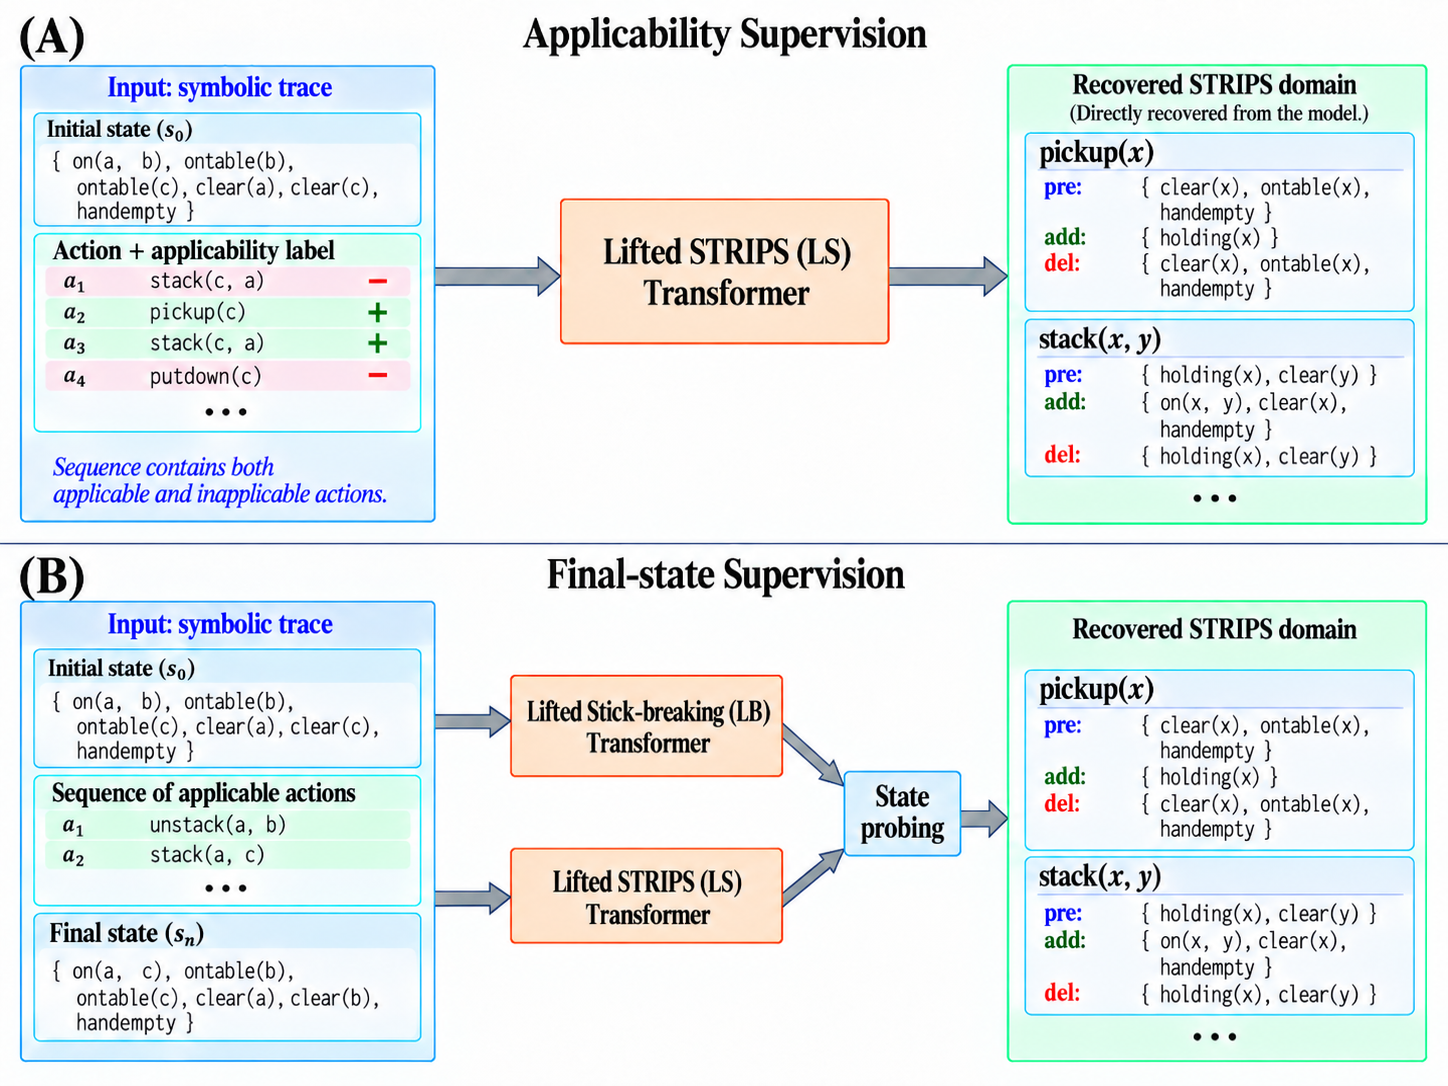
\includegraphics[width=\textwidth]{combined2_A.png}
%    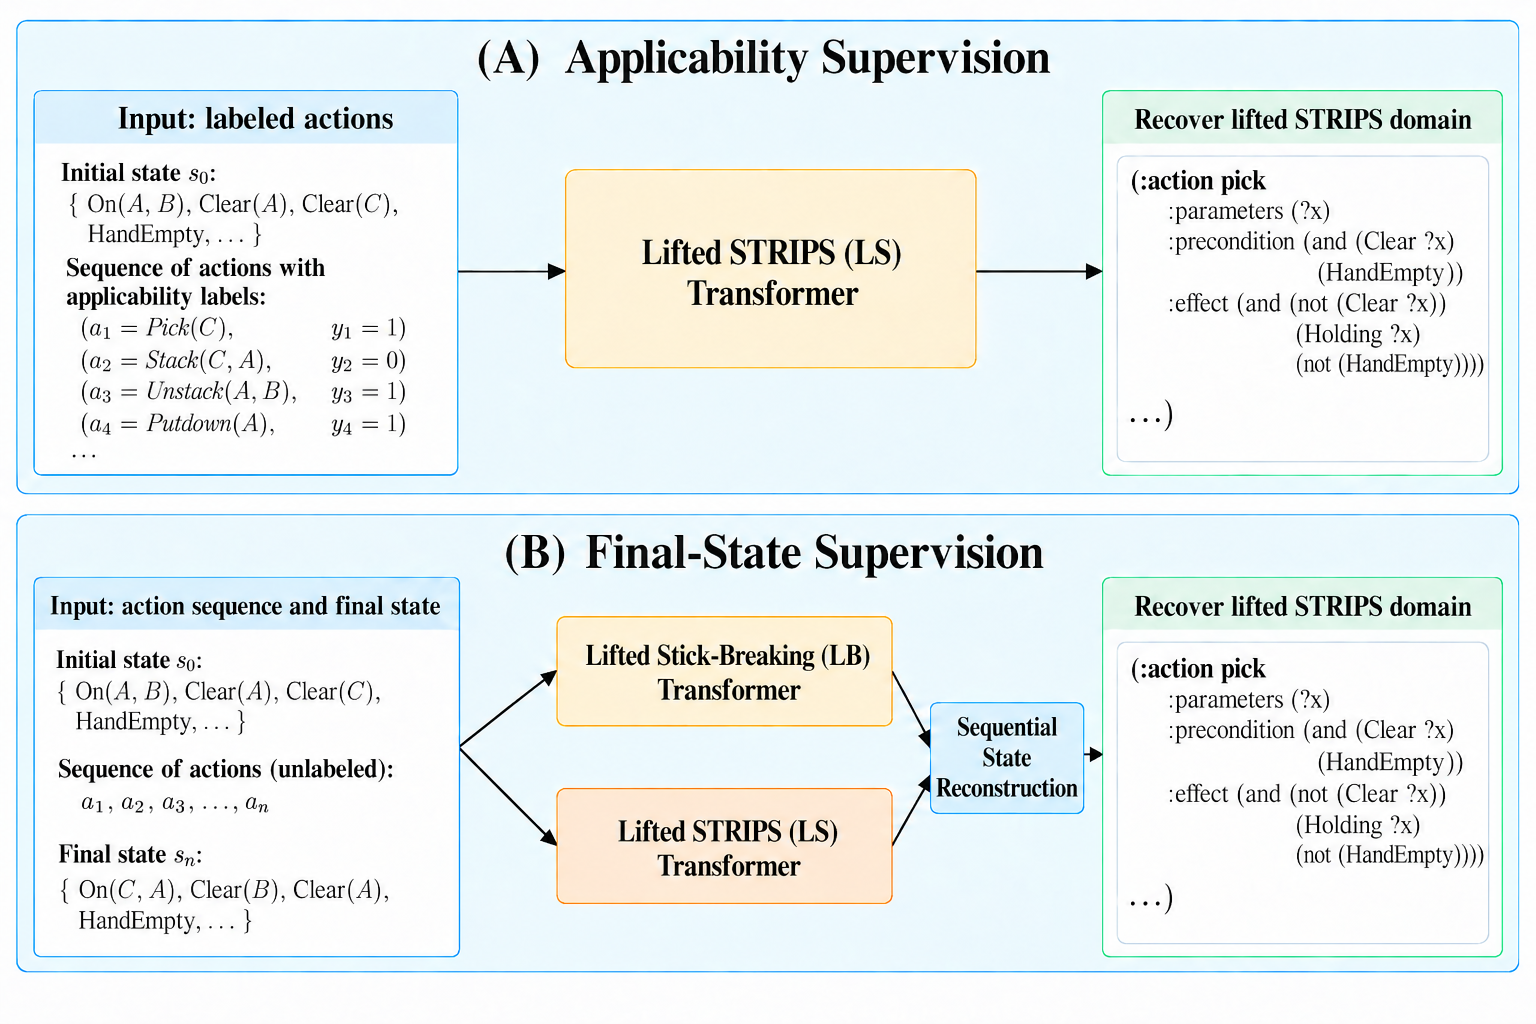
\includegraphics[width=\textwidth]{combined3_A.png}
%    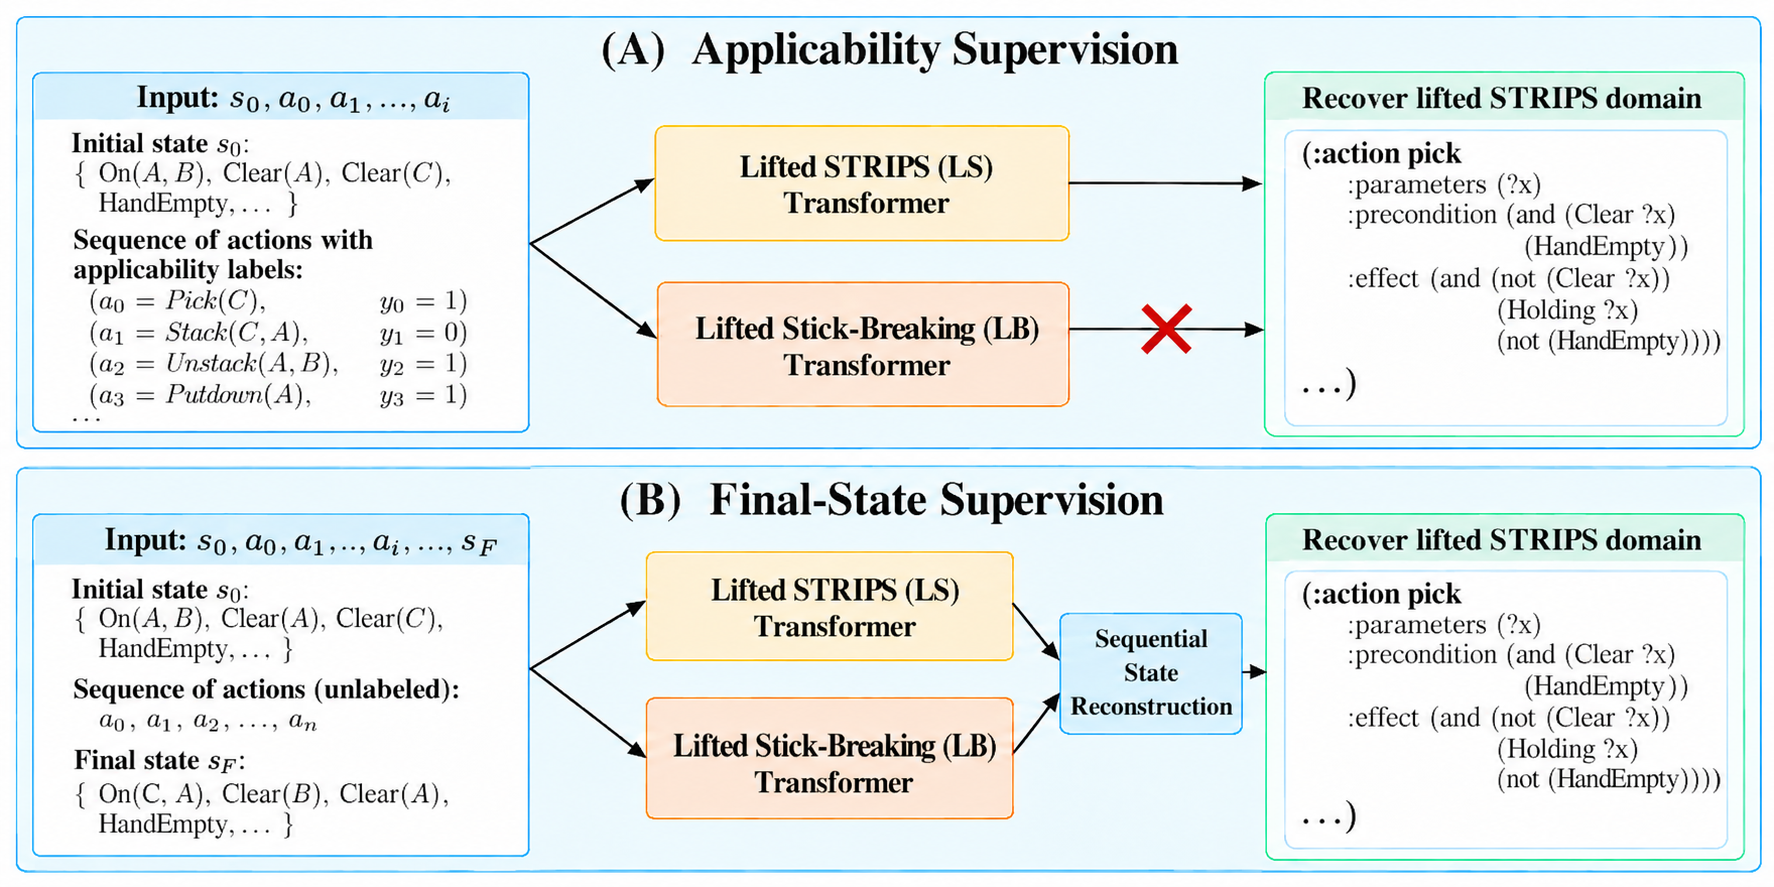
\includegraphics[width=\textwidth]{combined4_A.png}
    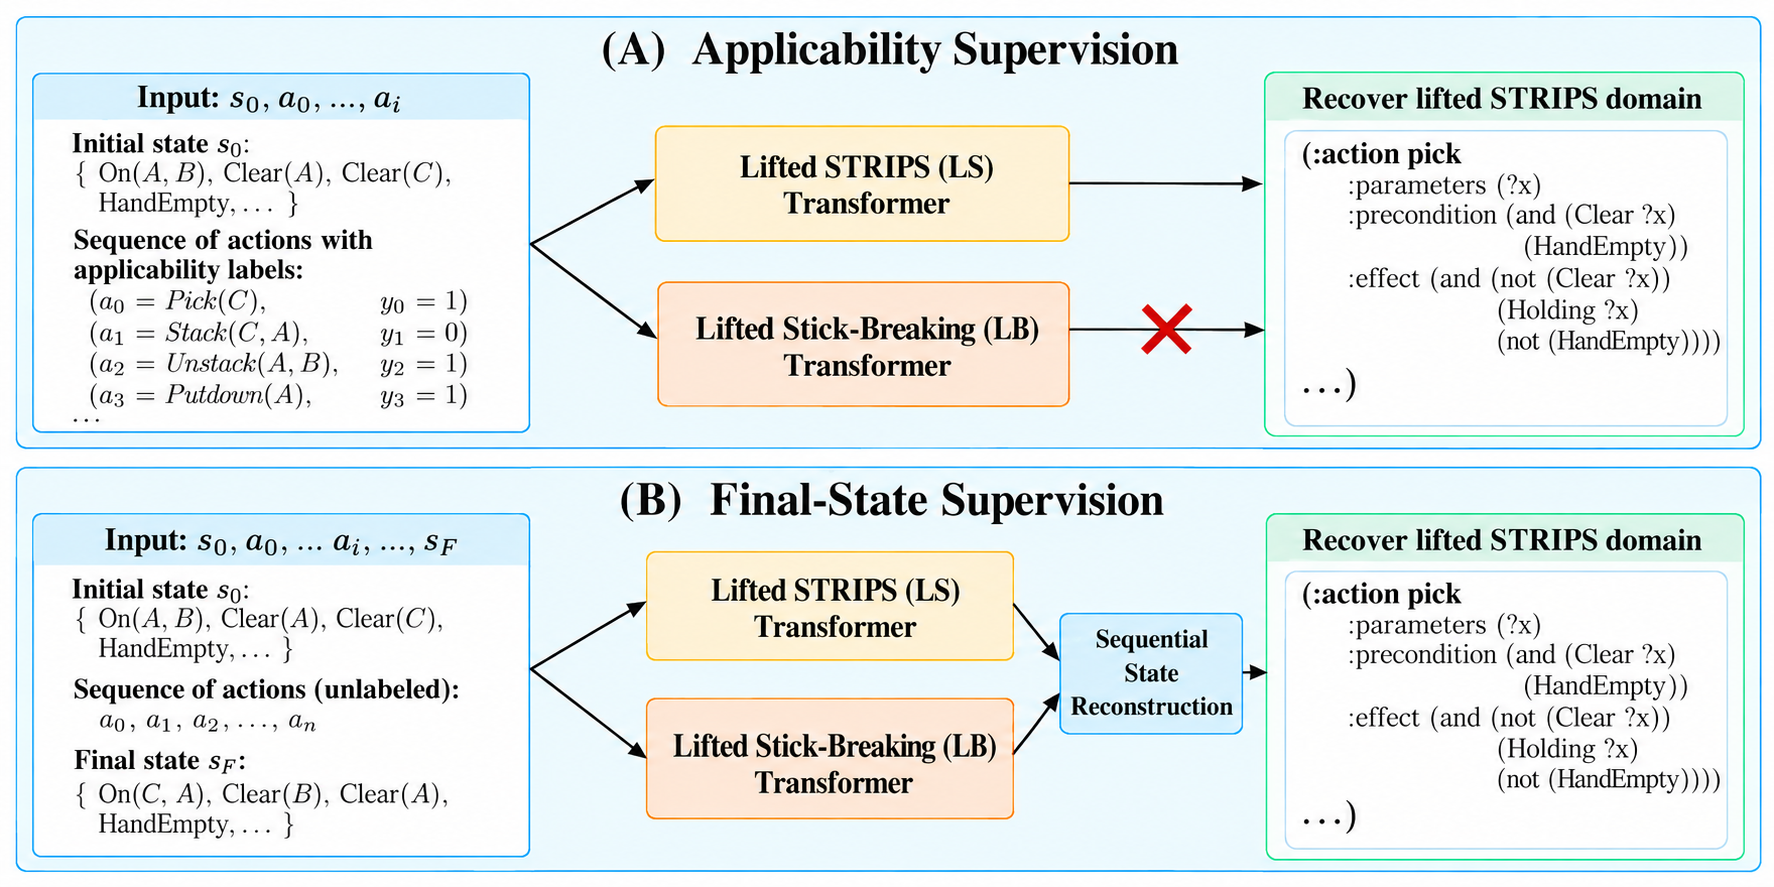
\includegraphics[width=\textwidth]{combined5_A.png}
\caption{ 
\textbf{Overview of the two architectures and supervision settings.}
We introduce the Lifted \strips (LS) Transformer, whose learned parameters are explicitly aligned with a symbolic action model, and the Lifted Stick-Breaking (LB) Transformer, an architecture closer to the standard Transformer that uses stick-breaking attention and randomized object embeddings. Both are trained from traces, each containing at least an initial state and an action sequence.
\textbf{(A) Applicability supervision:} actions in each trace are labeled as applicable or inapplicable, without observing any subsequent state. Only the Lifted \strips (LS) Transformer supports direct extraction of a symbolic action model from its learned parameters.
\textbf{(B) Final-state supervision:} each trace contains an initial state, an action sequence consisting only of applicable actions, and the resulting final state, but no applicability labels. A lifted symbolic model can be recovered from either architecture through a sequential state reconstruction procedure.
}
%         \caption{ \textbf{Overview of the two supervision settings.} \textbf{(A) Applicability supervision:} the model receives an initial state together with an action sequence whose actions are labeled as applicable or inapplicable. The Lifted \strips (LS) Transformer can be trained in this setting, and a symbolic action model can be extracted directly from its learned parameters. \textbf{(B) Final-state supervision:} the model receives an initial state, an applicable action sequence, and its resulting final state, but no applicability labels. In this more conventional setting, transformer variants can be trained, including the Lifted Stick-Breaking (LB) Transformer, which uses stick-breaking attention and randomized object embeddings, as well as the LS Transformer. A lifted symbolic model can then be recovered through a sequential state reconstruction procedure.        }
        \label{fig:applicability}
\end{figure*}
Our results show that both the LS and LB Transformers recover lifted world models that generalize to longer traces and to problem instances with more objects than those seen during training, whereas standard Transformer variants with softmax attention and positional encodings fail to recover the correct model. With final-state supervision, both architectures recover a \strips model through sequential state reconstruction, while with applicability supervision the LS Transformer recovers it directly, without observing any state after the initial one.

Our main contributions are:
\begin{itemize}
\item We introduce the Lifted \strips (LS) Transformer and the Lifted Stick-Breaking (SB) Transformer, \textbf{two transformer architectures for lifted world-model learning} with different structural biases and trade-offs.
\item We provide a \textbf{B-RASP formulation of lifted \strips trace recognition} and show that the LS Transformer provides a differentiable realization of this computation.
\item We study \textbf{two complementary forms of supervision} that trade off different sources of information. Final-state supervision learns from executable action sequences together with their resulting final states, whereas applicability supervision uses applicable and inapplicable actions without observing any subsequent state.
\item Across five planning domains, we demonstrate \textbf{generalization to substantially longer traces and problem instances with more objects than seen during training}. The LS Transformer achieves perfect generalization in the final-state setting and yields explicit lifted models that can be used for planning.
\end{itemize}
%\textbf{Carlos -- Provide main features/advantages of each transformer.}

%STRIPS Transformer. Parameters are continuous/soft approximation of lifted STRIPS models. Thus, there is one-to-one correspondence between quantized/binarized parameters and lifted STRIPS models. Also, to the best of our knowledge, it is the only Deep Learning-based method capable of learning world models without observing state transitions (\textit{risky claim, but I think it is true and an important contribution}).

%SB Transformer. Based on standard soft-attention transformer. Inspired by vector-symbolic architectures. Object tokens as non-learnable random embeddings. This forces the transformer to learn \textit{lifted equality} $x==y$, regardless of the particular objects $x,y$ represent. Therefore, it exhibits object generalization \textit{by design}.

% expand abstract ; picture of basic learning task, architecture, ...
%- Perhaps a Preview Section: concrete inputs, outputs

%In recent years, many works have considered whether transformers, and LLMs by extension, can learn world models as a result of performing next-token prediction. In this paper, we focus on world models expressed in STRIPS, a formal language based on first-order logic.

%STRIPS models possess two main advantages over neural world models. First, they are fully interpretable, since they are encoded as a set of logic rules. Second, they are lifted, meaning they generalize to tasks with any number of objects.

%We consider two alternative learning settings. In the applicability setting, each training trace encodes its initial state and a sequence of applicable and inapplicable actions, but contains no information about successor states. In the state prediction setting, traces encode their initial and final states, but do not include inapplicable actions.

%We perform experiments on five classical planning domains using both learning settings and transformers. Results show both transformers learn successfully across all domains. They achieve high training and test accuracy, generalizing to both longer traces and tasks with more objects. Additionally, they exhibit robust reasoning capabilities, as the extracted STRIPS models support planning via off-the-shelf symbolic algorithms.


\section{Related Work}

\noindent \textbf{Transformers and World Models}.
Work on chess and Othello has examined whether transformers trained for next-token prediction track and internally represent the underlying board state using state-tracking, probing, and interventions~\citep{Toshniwal_Wiseman_Livescu_Gimpel_2022,li_iclr,nanda2023linear}.
In maze-solving tasks, \citet{spies2025transformers} study internal representations of maze connectivity when the connectivity graph is provided
as input. 
Recent work has investigated whether causal structure can be recovered from transformer attention~\citep{rohekar2025a}.
Beyond state representations, \citet{world-models2} ask whether generative models recover the underlying transition structure, while \citet{vafa2025what} study whether predictive models acquire inductive biases that transfer to new tasks.
Another line learns symbolic world models for robot planning from perceptual observations, using neuro-symbolic abstractions and pretrained vision-language models
\citep{liang2025visualpredicator,liang2026exopredicator,athalye2026pixels}.
In contrast, we recover an explicit lifted \strips model rather than probe an implicit world model from symbolic traces without intermediate-state observations. In our applicability setting, no successor states are observed at all. We evaluate the resulting models through prediction and planning, including generalization to longer traces and larger object sets.


\noindent \textbf{Formal Languages and Transformer Generalization}.
To formally characterize computations performed by transformers, \citet{rasp} proposed a simple abstract programming language called RASP. \citet{yang2024masked} later developed a Boolean variant, B-RASP, and showed that masked hard-attention transformers characterize exactly the class of star-free languages. This connection is directly relevant to planning, since the set of valid action sequences in a \strips planning domain also forms a star-free language \citep{Lin_Bercher_2022}, implying that masked hard-attention transformers are expressive enough to recognize such sequences.

More recently, the C-RASP framework, an extension of RASP with counting operations, was introduced to study length generalization in soft-attention transformers~\citep{yang2024counting,huang2025length}.
Later, \citet{sarrof2026verify} extended this framework to C*-RASP to analyze plan verification in lifted \strips, where plan length and the number of objects increase at test time.
In contrast, our goal is not plan verification itself, but learning the underlying lifted \strips model. We use plan verification as an intermediate step toward this goal, building on B-RASP rather than C-RASP.

% -- Previous, I have removed the mention to well-formed domains
%They show that soft-attention transformers can verify \strips plans, but only for well-formed domains.
%By contrast, we show that B-RASP and, by extension, our proposed hard-attention transformers can recognize \strips without assuming that the domain is well-formed. %Moreover, we extract \strips models from the trained transformers.

% Carlos - no me gusta este párrafo porque "without the additional counting machinery" parece que indica que C-RASP es más complejo que B-RASP, cuando simplemente son complementarios. Nuestro acercamiento tiene dos ventajas sobre \ref{sarrof2026verify}: (1) B-RASP/hard-attention transformers no están limitados a well-formed STRIPS; (2) nosotros no solo verificamos planes, sino que extraemos el STRIPS domain del transformer.
%~\cite{sarrof2026verify} further extended this framework to C*-RASP to analyze plan verification when plan length and the number of objects increase at test time.
% Our analysis remains within B-RASP. We show that B-RASP already suffices to recognize lifted STRIPS traces involving a finite number of objects without requiring the additional counting machinery of C-RASP.

\noindent \textbf{Learning Action Models for Planning}.
Learning action models from trajectories has a long history in AI planning, with methods using fully or partially observed state-action sequences \citep{zhuo2013action,aineto2019learning,lamanna2025lifted} and others recovering lifted rules from action sequences alone \citep{locm,sift}. Recent work studies how much information about states and actions can be removed while still identifying the underlying dynamics \citep{jansen2025incomplete,gosgens2026minimal}. Neural approaches have also been used to learn propositional or lifted action models \citep{asai:jair,xi2024neuro,xi2026unsupervised,ajith2026strips}. 
% In contrast, we study action-model learning as a transformer sequence-learning problem and analyze how final-state observations and action-applicability labels provide alternative forms of supervision for recovering the underlying action model.
Our work generalizes~\citet{nunez2026strips} to a lifted setting by learning lifted models from traces of different domain instances, and by learning from positive traces only labeled with the final states.
%. Our traces are still grounded, but the learned action model is lifted and generalizes across object identities, including to problem instances with more objects and previously unseen ground actions. We also consider final-state prediction from positive traces alone, while \citet{nunez2026strips} requires negative actions for learning.
% learns from positive and negative traces using action-applicability labels only.

\noindent \textbf{Pre-trained LLMs and Symbolic Planning Models}.
Recent work uses pre-trained LLMs to generate explicit symbolic models that can be used by classical planners. First approaches generate PDDL domain models from natural-language descriptions \citep{NEURIPS2023_f9f54762,oswald2024large}, while more recent work improves domain generation through test-time sampling and refinement \citep{yu2025symbolic}, or derives PDDL models from demonstrations and visual simulation \citep{huang2026onedemo,hao2026simulation}, or decomposes world modeling into action-applicability and state-transition prediction using separate LLMs \citep{xie-etal-2025-making}.
In contrast, we learn lifted action models directly from symbolic traces, without relying on pre-trained semantic knowledge or external simulation.
This is specially relevant since prior exposure to the corresponding domain dynamics or PDDL encodings cannot generally be ruled out in these approaches, whereas our models learn the dynamics solely from the traces provided.


\section{Background}

\subsection{\strips Models}

A \strips model $M=\langle\mathcal{P},A\rangle$ consists of a finite set of predicates $\mathcal{P}$ and action schemas $A$~\citep{russell:book,ghallab:book,geffner:book}. Each predicate $p\in\mathcal{P}$ denotes a relation over objects with fixed arity $\operatorname{ar}(p)$. Each action schema $\alpha(x_1,\ldots,x_k)\in A$, with variables $x_1,\ldots,x_k$, specifies its preconditions $\mathrm{pre}(\alpha)$, add effects $\mathrm{add}(\alpha)$, and delete effects $\mathrm{del}(\alpha)$. We use untyped \strips, representing object types when needed by unary predicates. % such as $\mathrm{is\_car}(x)$.

A problem instance $P=\langle M,O_N,I,G\rangle$ specifies a model $M$, a finite object set $O_N={o_1,\ldots,o_N}$, an initial state $I$, and a goal $G$. Grounding variables with objects in $O_N$ yields ground atoms and ground actions $a=\alpha(o_1,\ldots,o_k),$ with corresponding grounded preconditions and effects. Both $I$ and $G$ are sets of ground atoms.

A problem instance defines a deterministic state-transition model, which can be viewed as the dynamics of a deterministic MDP over Boolean state variables. A state $s$ represents a truth-valuation over the ground atoms represented by those which are true in $s$. A ground action $a$ is applicable in $s$ when $\mathrm{pre}(a)\subseteq s$, and maps it to $s'=(s\cup\mathrm{add}(a))\setminus\mathrm{del}(a).$

An action trace $\tau=(a_0,\ldots,a_{n-1})$ is applicable from $s$ if each $a_i$ is applicable in the state reached from $s$ after executing $a_0,\ldots,a_{i-1}$. It is a plan for $P$ if it is applicable from $I$ and its resulting state contains $G$.

Since $M$ is lifted, its predicates and action schemas are independent of $O_N$, so the same model can be instantiated over problem instances with different numbers of objects.

\subsection{Transformers and Attention}
\label{sec:attention-background}

A Transformer~\cite{transformers} maps a sequence of token representations $(h_0,\ldots,h_{n-1})$ into contextual representations using self-attention and position-wise transformations. In an attention head, each representation is projected into a query $Q(i)$, key $K(i)$, and value $V(i)$, with attention score $S(i,j)=Q(i)K(j)^\top.$ We use strict future masking, so position $i$ can attend only to positions $j<i$. Standard attention applies softmax to these scores and returns a weighted combination of the corresponding values.

In \emph{masked hard attention}, position $i$ instead selects a preceding position with maximal score, resolving ties in favor of the rightmost one. \brasp~\cite{yang2024masked} is a Boolean programming language that provides an equivalent abstract representation of masked hard-attention Transformers.

\emph{Stick-breaking attention}~\cite{tan2025scaling} provides a differentiable relaxation of this rightmost-selection mechanism. For scores $S(i,j)\in[0,1]$, $j<i$, it computes
$$ \widetilde S(i,j) = S(i,j) \prod_{k=j+1}^{i-1} \bigl(1-S(i,k)\bigr). $$
When the scores are binary, only the rightmost preceding position with score $1$ receives nonzero weight, recovering masked hard attention.

\section{Learning Tasks}
\label{sec:task}

We consider two tasks for learning an unknown lifted \strips model
$M=\langle\mathcal{P},A\rangle$ from traces drawn from problem instances
$P=\langle M,O_N,I,G\rangle$. In both cases, a trace contains an initial
state $s_0=I$ and a sequence $\tau=(a_0,\ldots,a_{n-1})$ of ground actions
obtained by instantiating the action schemas in $A$ with objects from $O_N$.
The two tasks differ in the supervision provided with these traces.

\subsection{Applicability Supervision}

In this setting, every action $a_i$ in the trace is labeled as applicable or
inapplicable given $s_0$ and the preceding actions. Action $a_0$ is applicable
when its preconditions hold in $s_0$, while $a_i$, for $i>0$, is applicable
when its preconditions hold in the state obtained from $s_0$ after processing
$a_0,\ldots,a_{i-1}$.

To define labels after an inapplicable action, we treat such actions as
no-ops: they leave the current state unchanged. Thus, applicable actions
update the state according to $M$, whereas inapplicable actions do not affect
subsequent applicability. A trace is \emph{positive} if all its actions are
applicable and \emph{negative} otherwise.

Note that, effectively, each labeled sequence represents a collection of traces.
For every position $i$, removing the preceding inapplicable actions yields an applicable prefix;
appending $a_i$ to this prefix gives a positive trace if $a_i$ is applicable and a negative trace otherwise.
In our experiments, these labeled sequences are generated by random
exploration while keeping applicable and inapplicable examples balanced.

For a sequence $\tau_i=(a_0,\ldots,a_i)$, we define
$$ f_M(s_0,\tau_i)=
\begin{cases}
0, & \text{if $a_i$ is applicable after processing $a_0,\ldots,a_{i-1}$},\\
1, & \text{otherwise}.
\end{cases} $$
Here, preceding inapplicable actions are processed as no-ops, as described
above. The learning task is to learn a parametrized function
$f_\theta(s_0,\tau_i)$ that approximates $f_M$.

\subsection{Final-State Supervision}

This second setting is closer to world-model learning through state
prediction~\citep{world-models2,xie-etal-2025-making,spies2025transformers}.
In this setting, each trace consists of an initial state $s_0$, an applicable action sequence
$\tau=(a_0,\ldots,a_{n-1})$, and the final state $s_F$ reached by executing
$\tau$ from $s_0$. Intermediate states are not observed.

The Transformer is trained autoregressively by next-token prediction over
the complete sequence containing $s_0$, $\tau$, and $s_F$. Thus, predicting
the final-state tokens requires capturing the cumulative effects of the
actions in the trace, without direct supervision of the intermediate state
transitions.

% Vicenc: maybe add more here?

\section{Transformer Architectures}
\label{sec:arch}


\textbf{Carlos - comentar que applicability supervision sería aplicable al LB transformer también pero, como no podemos hacer symbolic alignment, no se podría extraer \strips model. Por tanto, en nuestros experimentos no usamos applicability supervision con LB.}

can remove the need for final-state observations (no goal actions) -\> STRIPS Transformer
(first method that does not require transitions PDDL) value (tambien conexion con B-RASP and alignment

\noindent
\begin{minipage}[t]{0.53\textwidth}
\vspace{0pt}
    \centering
    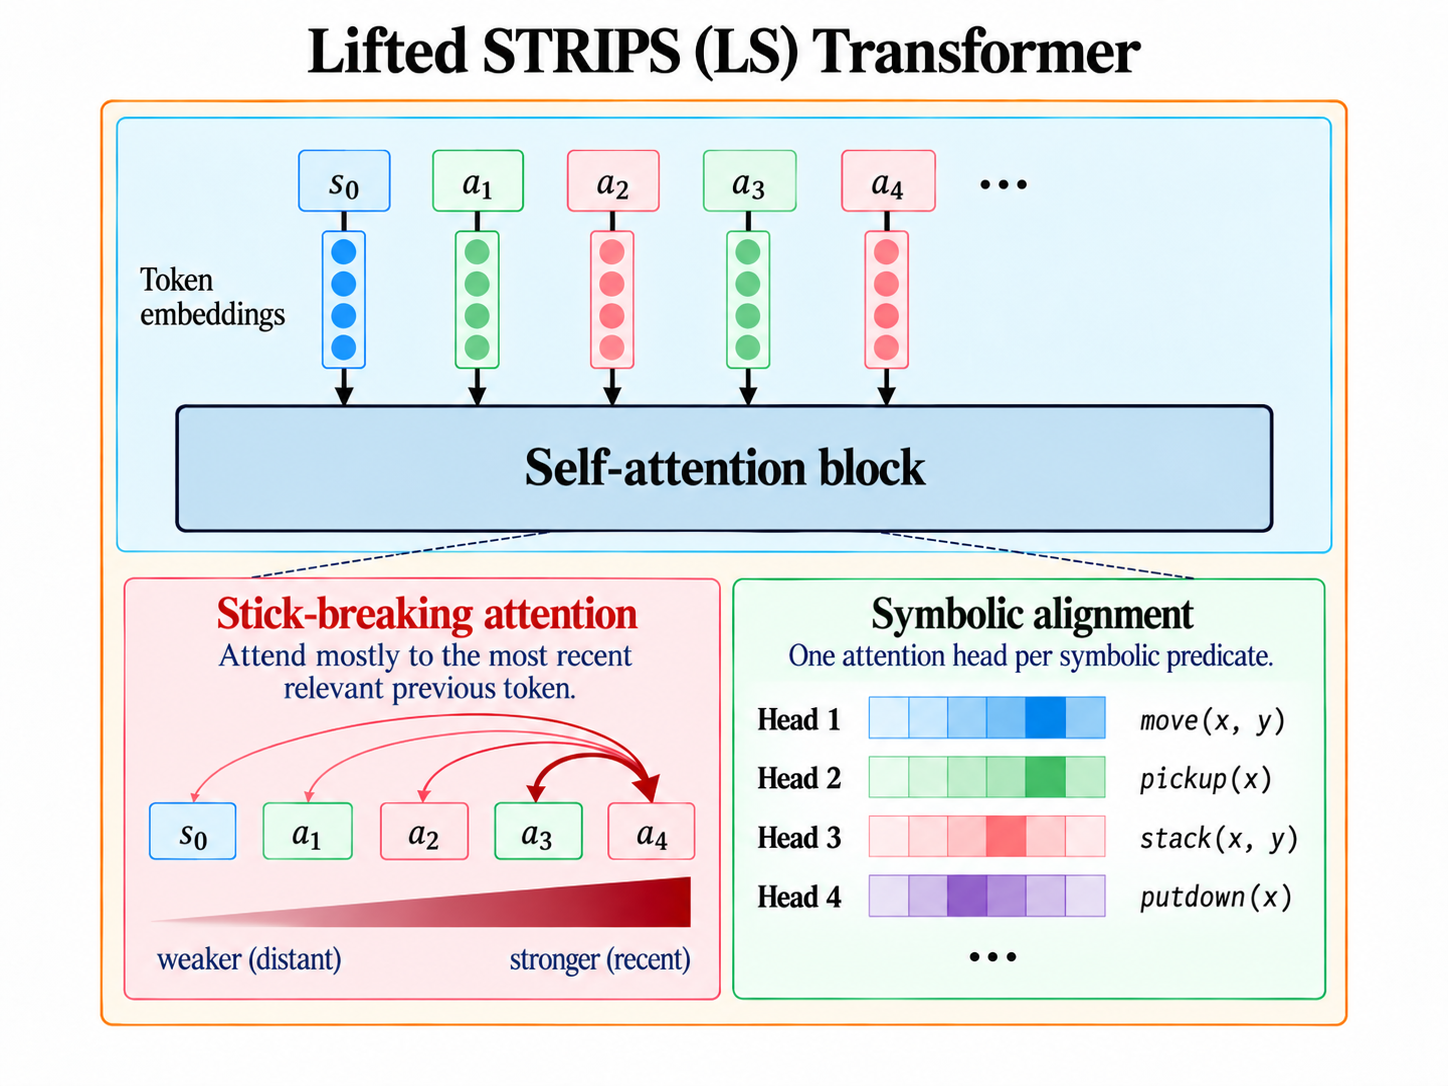
\includegraphics[width=\linewidth]{LS_transformer.png}
    \captionof{figure}{Architecture of the Lifted \strips Transformer.}
    \label{fig:ls-transformer}
\end{minipage}
\hfill
\begin{minipage}[t]{0.48\textwidth}
\vspace{0pt}
    The architecture ...
    
    The attention heads ...
    
    The learned parameters ...    The architecture ...
    
    The attention heads ...
    
    The learned parameters ...    The architecture ...
    
    The attention heads ...
    
    The learned parameters ...
\end{minipage}


\subsection{Final State Supervision}

can remove the need for negative examples (only positive actions + goal actions) -> SB Transformer   rosame (intermedio imágenes)





\textbf{Carlos -- for the SB Transformer, we use a special separator token <sep> between actions. Labels are associated with the SEP token after each action, so the transformer uses that token to predict applicability for domain/goal actions.}

\textbf{Carlos -- The process for extracting the STRIPS model from the transformers is explained in the overleaf document, section 16.11. The method for applicability supervision is in Section 16.11.1, and for state supervision in 16.11.2.}

State prediction, SB transf, Randomized Obj Embeds

Transformers can learn lifted symbolic world models from action traces that generalize simultaneously to longer horizons and to larger numbers of objects. Moreover, different forms of supervision can substitute for one another: with final-state observations, positive action traces suffice. With action-applicability supervision, final-state observations can sometimes be dispensed with altogether.




\section{Experiments}

\label{sec:experiments}
% >> TODO - add appendix with PDDL domains, generator params., transformer hyperparameters (num layers, batch size, lr, bce/goal-bce weight, focal coeff, dropout,), num predicates LS Transformer for each domain (GT conf.), <Explain how parameters \theta of LS Transformer preconds and effects are initialized! Also explain gumbel sigmoid temp> etc.
% Also --weight-init-method z (how LS Transformer params are initialized)
Our experiments address the following research questions:
\begin{itemize}
    \item[\textbf{RQ1:}] How do the LS and LB Transformers compare against standard transformer baselines?
    \item[\textbf{RQ2:}] How does symbolic alignment affect performance under final-state supervision, and how does the supervision setting affect the LS Transformer?
    \item[\textbf{RQ3:}] Can the trained transformers yield explicit \strips models that support planning?
    \item[\textbf{RQ4:}] Do the learned models extrapolate to longer traces and larger object sets?
\end{itemize}
%We explain our experimental setup below.
\paragraph{Baselines.}
We compare our models with two softmax-attention Transformer baselines:
\textbf{Sinusoidal}, using sinusoidal positional encodings
\citep{transformers}, and
\textbf{RoPE}, using rotary position embeddings
\citep{su2024roformer}, which can improve length generalization
\citep{spies2025transformers}.
Both use the same tokenization, randomized object embeddings, and network
dimensions as LB.
Positional information is applied to half of each token embedding to separate
it partially from the randomized object representation.
% \paragraph{Baselines.}
% We compare our proposed models against two standard baselines: \textbf{sinusoidal}, the original soft-attention transformer \citep{transformers}, with softmax aggregation and sinusoidal positional encodings; and \textbf{RoPE}, a soft-attention transformer with softmax aggregation and Rotary Position Embeddings \citep{su2024roformer}, which have been shown to improve generalization on longer sequences \citep{spies2025transformers}. 
%In both, positional information is applied only to half of each token embedding, to partially separate positional information from the randomized object embeddings.
\paragraph{Planning domains.}
We evaluate on standard automated-planning domains
\citep{long20033rd,fern2011first,taitler20242023}:
\textbf{\bw} (block rearrangement),
\textbf{\fr} (car transport by ferry),
\textbf{\lgt} (package delivery),
\textbf{\np} (sliding tiles), and
\textbf{\mz} (grid navigation).


% > Removed bullet points for space
\iffalse
In both, positional information is applied only to half of each token embedding, to partially separate positional information from the randomized object embeddings.

\begin{itemize}
    \item \textbf{Sinusoidal}: the original soft-attention transformer architecture proposed in \citep{transformers}, using softmax aggregation and sinusoidal positional encodings.
    \item \textbf{RoPE}: a soft-attention transformer with softmax aggregation and Rotary Position Embeddings \citep{su2024roformer}, which have been shown to improve generalization on longer sequences \citep{spies2025transformers}.
\end{itemize}

\paragraph{Planning domains.}
We perform experiments on five planning domains widely used in the AP community \citep{long20033rd,fern2011first,taitler20242023}:
\textbf{\bw}, where a set of blocks must be reassembled into a target configuration with a robotic gripper;
\textbf{\fr}, where a ferry is used to transport cars between different ports;
\textbf{\lgt}, a logistics task where a fleet of trucks and airplanes is used to deliver packages across locations in different cities;
\textbf{\np}, a puzzle where numbered tiles must be slid into their goal positions;
\textbf{\mz}, where an agent must traverse a grid-based maze to reach a goal location.
\fi

\paragraph{Data generation.}
For each domain, we generate 100 problems for each of the training, test, and planning splits using randomized generators.
Test and planning problems contain more objects than training problems. Training and test problems generate random traces whose numbers of domain actions are sampled uniformly from $[1,D]$. We generate $10^5$ training traces with $D=50$ and
$2\cdot10^5$ test traces with $D=200$. Exact object counts are reported in Appendix~\ref{app:problems}.

Under applicability supervision, each training action is sampled as applicable or inapplicable with equal probability. At test time, the prefix contains only applicable actions and only the final domain action may be inapplicable. Under final-state supervision, all domain actions are applicable, and each trace contains ten ground-atom queries sampled uniformly from all ground atoms over $O$.

\paragraph{Training and evaluation.}
The LS and LB Transformers are trained with Adam~\citep{liu2019variance}. We use $10^5$ training steps for LS and $5\cdot10^5$ for LB, increasing the latter to $7.5\cdot10^5$ in \lgt. Every $10^4$ steps, we compute accuracy on the full training set and retain the checkpoint with the highest training accuracy. We run each configuration with five random seeds and report mean performance, with the result of the seed achieving the highest training accuracy in parentheses.

Trace accuracy is the percentage of traces for which all supervised labels are predicted correctly. Under applicability supervision, these are the domain-action labels. Under final-state supervision, they are the final-state query labels. LS predictions use the binarized parameters $\bar{\theta}$, while LB
predictions are thresholded at $0.5$.
For RQ4, we vary trace length and object count, keeping the other dimension at its largest training value. We evaluate $10^4$ traces per setting and report the seed with the highest training accuracy.
We extract \strips models using the procedure associated with each supervision setting.
Planning accuracy is the percentage of planning problems for which the planner returns, within the search budget, a plan that is valid under the ground-truth model. All experiments run on an NVIDIA L40S GPU and an Intel Xeon Gold 6542Y CPU. Appendix~\ref{app:configuration} provides additional configuration details and model hyperparameters.

%\paragraph{Training and evaluation.}
%Both architectures are trained with RAdam \citep{liu2019variance}, using $10^5$ steps for the LS Transformer and $5\cdot10^5$ for the LB Transformer, increasing to $7.5\cdot10^5$ steps in \lgt for the latter.
%We perform validation every $10^4$ training steps, computing accuracy on the whole training dataset. After training, the checkpoint with the highest accuracy is tested. Accuracy is measured as the percentage of traces correctly classified, where a trace is considered correct only if the transformer correctly predicts the applicability label of each action in the trace. For the LS Transformer, predictions are obtained using the binarized parameters $\bar{\theta}$, whereas for the LB Transformer predictions are rounded to $\{0,1\}$.
%We extract \strips models from both architectures for planning, with the procedure corresponding to the supervision setting. Then, planning accuracy is computed as the percentage of planning problems correctly solved with the extracted model, i.e., those for which the planner outputs a valid plan.
%Finally, each experiment is conducted on a machine with an NVIDIA L40S GPU and an Intel Xeon Gold 6542Y CPU.
% If we don't say it before, say that we use GBFS FF and pymimir for planning!

\section{Results}
\begin{table}[t]
\centering
\setlength{\tabcolsep}{4pt}
\caption{\textbf{Main results.}
Comparison of LS Transformer, LB Transformer and baseline models across five domains and two supervision settings, \textit{final-state} and \textit{applicability}, where the latter is only used by the LS Transformer. We report average training, test, and planning
accuracy across five seeds, with the result of the seed achieving the highest training accuracy in parentheses. For the LS Transformer, we consider both the number of predicates in the ground-truth domain (\textit{GT}) and a larger number of predicates shared across domains (\textit{Shared}). Perfect values are highlighted in bold.}
\label{tab:main-results}
\vspace{\baselineskip}

% Blocksworld
\begin{tabular*}{\linewidth}{@{\extracolsep{\fill}}lcccccc@{}}
\toprule
\multicolumn{7}{c}{\textbf{Blocksworld}} \\
\midrule
& \multicolumn{3}{c}{Final-state supervision} & \multicolumn{3}{c}{Applicability supervision} \\
\cmidrule(lr){2-4}\cmidrule(lr){5-7}
Model & Train & Test & Plan & Train & Test & Plan \\
\midrule
LS GT
& $\mathbf{1.0}$ $(\mathbf{1.0})$
& $\mathbf{1.0}$ $(\mathbf{1.0})$
& $\mathbf{1.0}$ $(\mathbf{1.0})$
& .439 $(\mathbf{1.0})$
& .405 $(\mathbf{1.0})$
& .238 $(\mathbf{1.0})$ \\
LS Shared
& $\mathbf{1.0}$ $(\mathbf{1.0})$
& $\mathbf{1.0}$ $(\mathbf{1.0})$
& $\mathbf{1.0}$ $(\mathbf{1.0})$
& .606 $(\mathbf{1.0})$
& .477 $(\mathbf{1.0})$
& .602 $(.020)$ \\
LB
& .995 $(.998)$
& .980 $(.991)$
& $\mathbf{1.0}$ $(\mathbf{1.0})$
& N/A
& N/A
& N/A \\
Sinusoidal
& .186 $(.186)$
& .457 $(.458)$
& 0.0 $(0.0)$
& N/A
& N/A
& N/A \\
RoPE
& .306 $(.328)$
& .419 $(.388)$
& 0.0 $(0.0)$
& N/A
& N/A
& N/A \\
\bottomrule
\end{tabular*}

\vspace{0.7em}

% Ferry
\begin{tabular*}{\linewidth}{@{\extracolsep{\fill}}lcccccc@{}}
\toprule
\multicolumn{7}{c}{\textbf{Ferry}} \\
\midrule
& \multicolumn{3}{c}{Final-state supervision} & \multicolumn{3}{c}{Applicability supervision} \\
\cmidrule(lr){2-4}\cmidrule(lr){5-7}
Model & Train & Test & Plan & Train & Test & Plan \\
\midrule
LS GT
& $\mathbf{1.0}$ $(\mathbf{1.0})$
& $\mathbf{1.0}$ $(\mathbf{1.0})$
& $\mathbf{1.0}$ $(\mathbf{1.0})$
& .700 $(\mathbf{1.0})$
& .627 $(\mathbf{1.0})$
& .600 $(\mathbf{1.0})$ \\
LS Shared
& $\mathbf{1.0}$ $(\mathbf{1.0})$
& $\mathbf{1.0}$ $(\mathbf{1.0})$
& $\mathbf{1.0}$ $(\mathbf{1.0})$
& .686 $(\mathbf{1.0})$
& .618 $(\mathbf{1.0})$
& .618 $(\mathbf{1.0})$ \\
LB
& .997 $(.999)$
& .993 $(.997)$
& $\mathbf{1.0}$ $(\mathbf{1.0})$
& N/A
& N/A
& N/A \\
Sinusoidal
& .410 $(.847)$
& .502 $(.635)$
& 0.0 $(0.0)$
& N/A
& N/A
& N/A \\
RoPE
& .799 $(.997)$
& .574 $(.678)$
& .200 $(\mathbf{1.0})$
& N/A
& N/A
& N/A \\
\bottomrule
\end{tabular*}

\vspace{0.7em}

% Logistics
\begin{tabular*}{\linewidth}{@{\extracolsep{\fill}}lcccccc@{}}
\toprule
\multicolumn{7}{c}{\textbf{Logistics}} \\
\midrule
& \multicolumn{3}{c}{Final-state supervision} & \multicolumn{3}{c}{Applicability supervision} \\
\cmidrule(lr){2-4}\cmidrule(lr){5-7}
Model & Train & Test & Plan & Train & Test & Plan \\
\midrule
LS GT
& $\mathbf{1.0}$ $(\mathbf{1.0})$
& $\mathbf{1.0}$ $(\mathbf{1.0})$
& $\mathbf{1.0}$ $(\mathbf{1.0})$
& 1.000 $(\mathbf{1.0})$
& 1.000 $(\mathbf{1.0})$
& .630 $(\mathbf{1.0})$ \\
LS Shared
& $\mathbf{1.0}$ $(\mathbf{1.0})$
& $\mathbf{1.0}$ $(\mathbf{1.0})$
& $\mathbf{1.0}$ $(\mathbf{1.0})$
& .958 $(\mathbf{1.0})$
& .769 $(\mathbf{1.0})$
& .614 $(\mathbf{1.0})$ \\
LB
& .971 $(.980)$
& .893 $(.903)$
& .010 $(.010)$
& N/A
& N/A
& N/A \\
Sinusoidal
& .529 $(.589)$
& .682 $(.680)$
& .010 $(.010)$
& N/A
& N/A
& N/A \\
RoPE
& .972 $(.978)$
& .401 $(.398)$
& .010 $(.010)$
& N/A
& N/A
& N/A \\
\bottomrule
\end{tabular*}

\end{table}

\begin{table}[t]
\centering
\setlength{\tabcolsep}{4pt}
\caption{\textbf{Continuation of Table \ref{tab:main-results}.}}
\label{tab:main-results-cont}
\vspace{\baselineskip}

% Npuzzle
\begin{tabular*}{\linewidth}{@{\extracolsep{\fill}}lcccccc@{}}
\toprule
\multicolumn{7}{c}{\textbf{Npuzzle}} \\
\midrule
& \multicolumn{3}{c}{Final-state supervision} & \multicolumn{3}{c}{Applicability supervision} \\
\cmidrule(lr){2-4}\cmidrule(lr){5-7}
Model & Train & Test & Plan & Train & Test & Plan \\
\midrule
LS GT
& $\mathbf{1.0}$ $(\mathbf{1.0})$
& $\mathbf{1.0}$ $(\mathbf{1.0})$
& $\mathbf{1.0}$ $(\mathbf{1.0})$
& $\mathbf{1.0}$ $(\mathbf{1.0})$
& $\mathbf{1.0}$ $(\mathbf{1.0})$
& .946 $(.980)$ \\
LS Shared
& $\mathbf{1.0}$ $(\mathbf{1.0})$
& $\mathbf{1.0}$ $(\mathbf{1.0})$
& $\mathbf{1.0}$ $(\mathbf{1.0})$
& .808 $(\mathbf{1.0})$
& .801 $(\mathbf{1.0})$
& .740 $(\mathbf{1.0})$ \\
LB
& .884 $(.992)$
& .889 $(.989)$
& .600 $(\mathbf{1.0})$
& N/A
& N/A
& N/A \\
Sinusoidal
& .356 $(.360)$
& .563 $(.563)$
& 0.0 $(0.0)$
& N/A
& N/A
& N/A \\
RoPE
& .386 $(.395)$
& .510 $(.470)$
& 0.0 $(0.0)$
& N/A
& N/A
& N/A \\
\bottomrule
\end{tabular*}

\vspace{0.7em}

% Mazefree
\begin{tabular*}{\linewidth}{@{\extracolsep{\fill}}lcccccc@{}}
\toprule
\multicolumn{7}{c}{\textbf{Maze}} \\
\midrule
& \multicolumn{3}{c}{Final-state supervision} & \multicolumn{3}{c}{Applicability supervision} \\
\cmidrule(lr){2-4}\cmidrule(lr){5-7}
Model & Train & Test & Plan & Train & Test & Plan \\
\midrule
LS GT
& $\mathbf{1.0}$ $(\mathbf{1.0})$
& $\mathbf{1.0}$ $(\mathbf{1.0})$
& $\mathbf{1.0}$ $(\mathbf{1.0})$
& .808 $(\mathbf{1.0})$
& .801 $(\mathbf{1.0})$
& .800 $(\mathbf{1.0})$ \\
LS Shared
& $\mathbf{1.0}$ $(\mathbf{1.0})$
& $\mathbf{1.0}$ $(\mathbf{1.0})$
& $\mathbf{1.0}$ $(\mathbf{1.0})$
& .615 $(\mathbf{1.0})$
& .602 $(\mathbf{1.0})$
& .600 $(\mathbf{1.0})$ \\
LB
& .981 $(.989)$
& .970 $(.981)$
& $\mathbf{1.0}$ $(\mathbf{1.0})$
& N/A
& N/A
& N/A \\
Sinusoidal
& .142 $(.186)$
& .122 $(.148)$
& $\mathbf{1.0}$ $(\mathbf{1.0})$
& N/A
& N/A
& N/A \\
RoPE
& .135 $(.249)$
& .126 $(.117)$
& .250 $(\mathbf{1.0})$
& N/A
& N/A
& N/A \\
\bottomrule
\end{tabular*}

\end{table}


\begin{figure}[t]
    \centering
    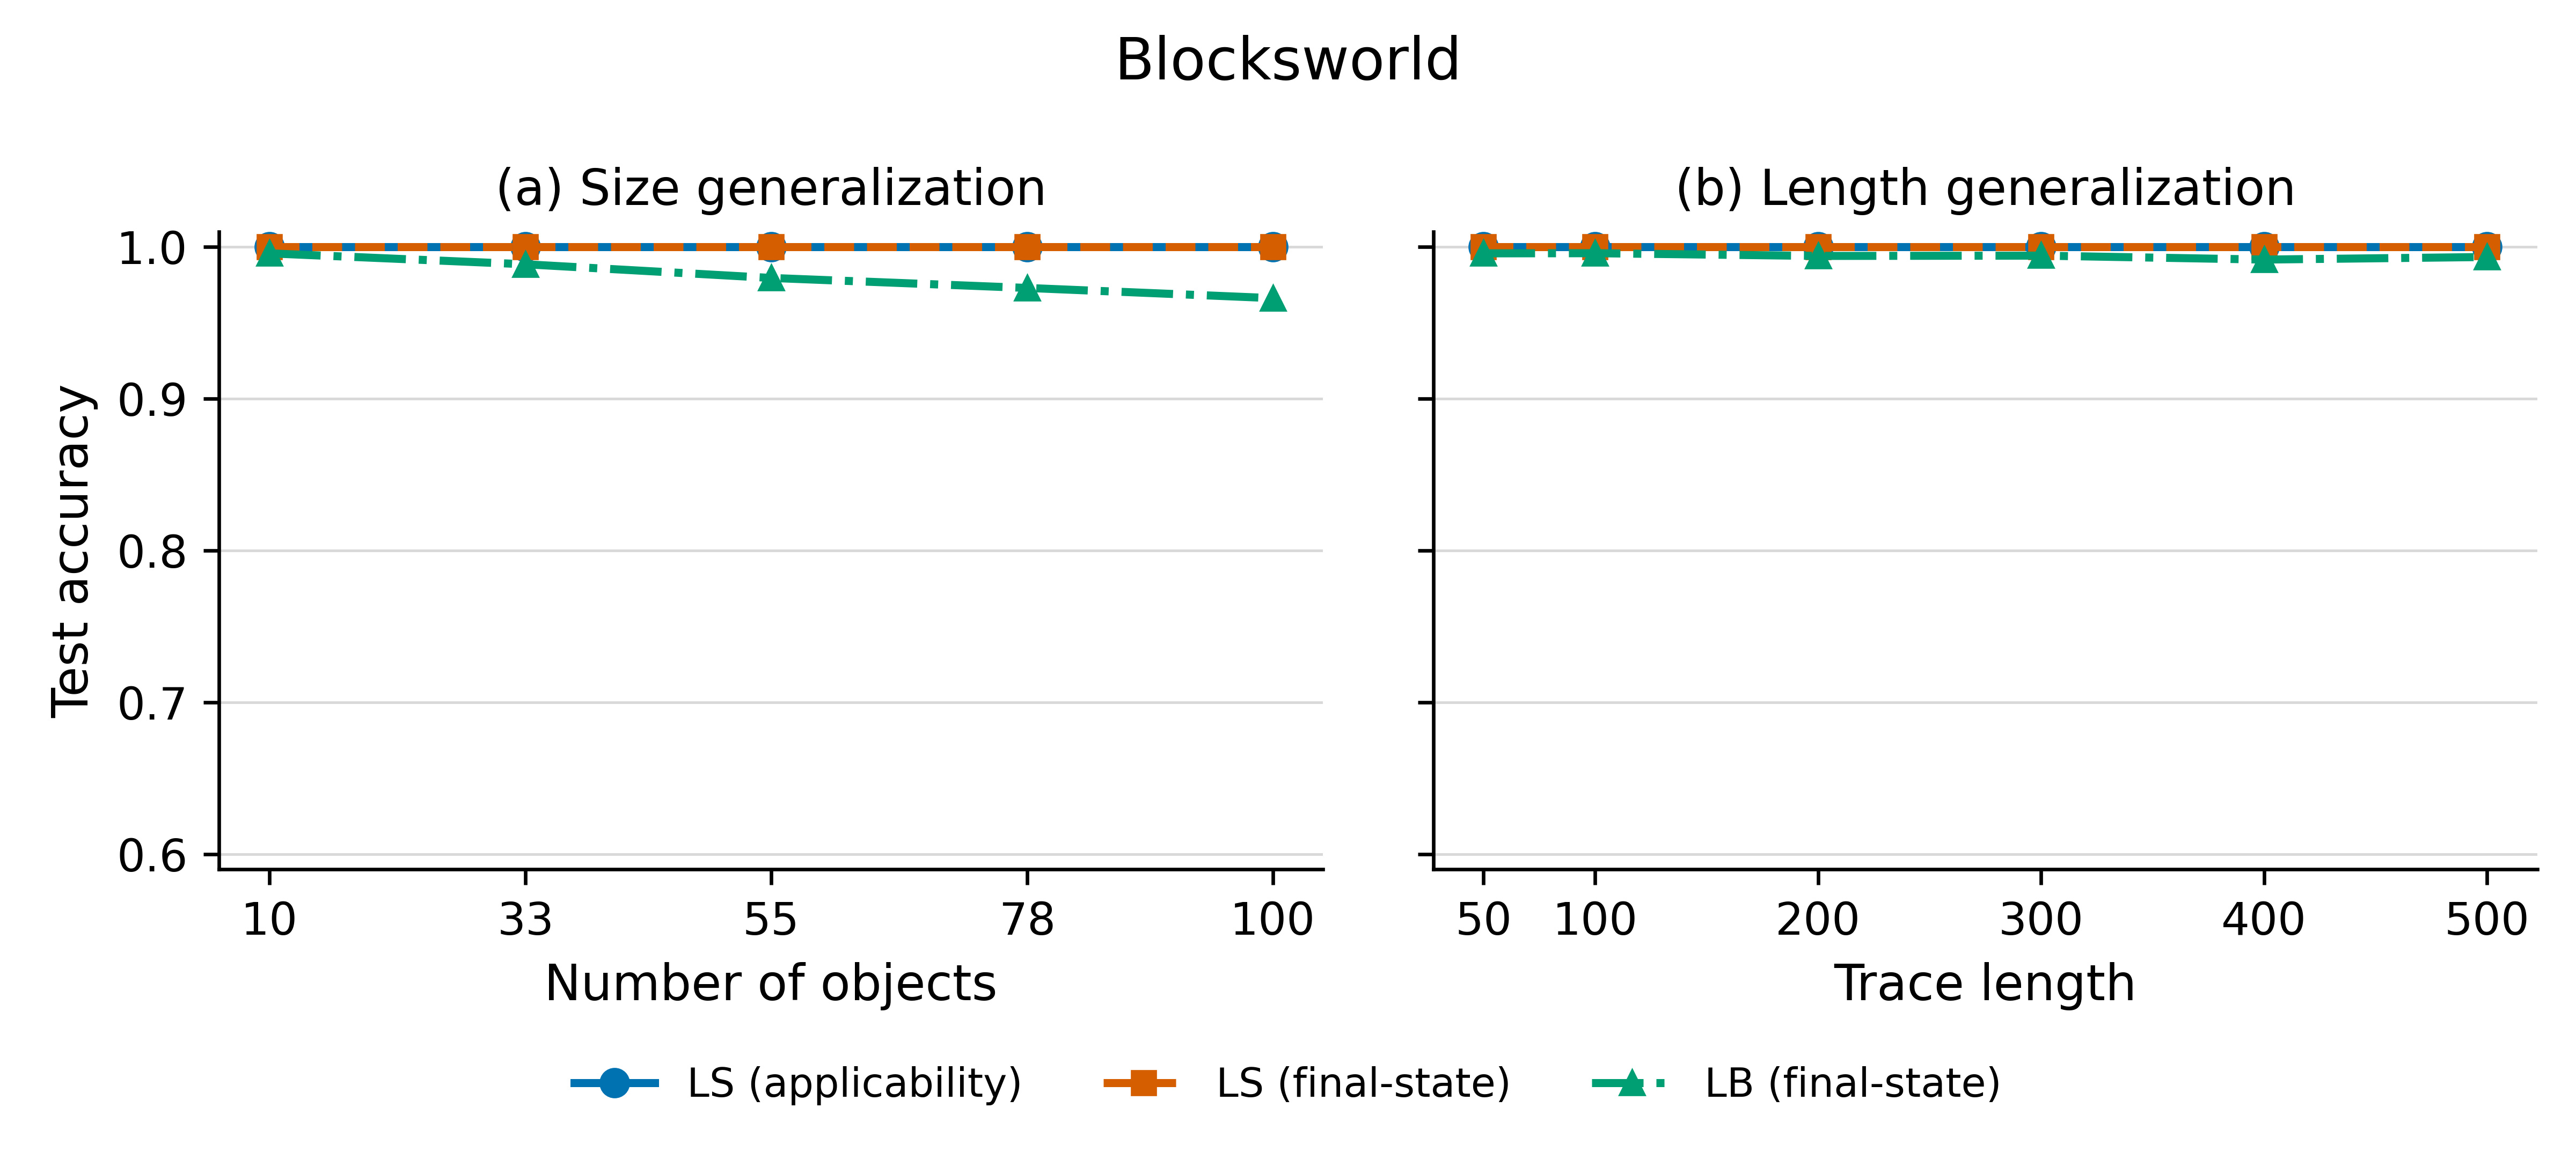
\includegraphics[width=\columnwidth]{imgs/gen_plot_blocksworld.jpg}
    \caption{\textbf{Generalization in \bw.}
    Plots show test accuracy for the \strips and LB Transformers when generalizing to
    \textbf{(a)} larger numbers of objects, up to $10\times$ the training size, while keeping trace length to the training value of $D=50$, and
    \textbf{(b)} longer traces, up to $10\times$ the training length, while keeping the number of objects to the largest value seen during training.
    For the LS Transformer, we use the shared predicate configuration from Tables~\ref{tab:main-results} and~\ref{tab:main-results-cont}, and report both supervision settings.
    To measure generalization subject to the model correctly fitting the training data, we report only the seed with the highest training accuracy.
    %For each model, we report only the seed with the highest training accuracy.
    The $y$-axis starts at $0.6$, and we use $10^4$ traces for each dataset.
    Results for the remaining domains are provided in Appendix~\ref{app:gen}.}
    \label{fig:bw-gen}
\end{figure}

\begingroup
\begin{figure*}[t]
\centering
\hrule height 0.8pt
\vspace{0.6em}
\noindent
% strips_gt_app: seed 1, training accuracy 1
\begin{minipage}[t]{0.33\textwidth}
\vspace{0pt}
{\centering (a) LS (applicability)\par}
\begin{lstlisting}
(:action stack
 :parameters (?x ?y)
 :precondition (and
  (clear ?x)
  (clear ?y)
  (ontable ?x)
  (p3 ?x))
 :effect (and
  (handempty)
  (on ?x ?y)
  (not (clear ?y))
  (not (ontable ?x))
  (not (p3 ?x))))
\end{lstlisting}
\end{minipage}\hfill%
% strips_gt_state: seed 1, training accuracy 1
\begin{minipage}[t]{0.33\textwidth}
\vspace{0pt}
{\centering (b) LS (final-state)\par}
\begin{lstlisting}
(:action stack
 :parameters (?x ?y)
 :precondition (and
  (clear ?y)
  (holding ?x))
 :effect (and
  (clear ?x)
  (handempty)
  (on ?x ?y)
  (not (clear ?y))
  (not (holding ?x))))
\end{lstlisting}
\end{minipage}\hfill%
% sb_state: seed 4, training accuracy 0.99782
\begin{minipage}[t]{0.33\textwidth}
\vspace{0pt}
{\centering (c) LB (final-state)\par}
\begin{lstlisting}
(:action stack
 :parameters (?x ?y)
 :precondition (and
  (clear ?y)
  (holding ?x))
 :effect (and
  (clear ?x)
  (handempty)
  (on ?x ?y)
  (not (clear ?y))
  (not (holding ?x))))
\end{lstlisting}
\end{minipage}%
\par\vspace{0.6em}
\hrule height 0.8pt
\captionsetup{position=bottom}
\captionof{lstlisting}{
\textbf{Fragment of extracted \strips models.}
Excerpts of the \strips models extracted from the LS and LB Transformers in \bw, showing the learned action schema \texttt{stack}.
Appendix \ref{app:strips-models} contains the full \strips models for each domain.
For the LS Transformer, we use the ground-truth predicate configuration from Tables~\ref{tab:main-results} and~\ref{tab:main-results-cont}, and report both supervision settings.
For each model, we select the seed with the best training accuracy.
In (a), predicate \texttt{p3} denotes a hidden predicate that cannot be aligned with a ground-truth predicate because it does not appear in the initial states. In this example, it encodes the predicate \texttt{holding}.
Finally, we note that the extracted models are fully interpretable.
}
\label{lst:blocksworld}
\end{figure*}
\endgroup

% ----------------------------- Analysis - answer Research Question

% TODO - no decir que applicability "no aplica" al SB Trans.

% Talk about SB Trans. planning failure in logistics (see email) -> data balancing issues, at(x,y) not present in preconditions...

% Mirar dominios extraidos appendix
% Mirar object generalization plots appendix


% Mention table 1
% Summarize results baselines vs LS/LB (do not focus on LS vs LB) -> focus on baselines vs LB
% Analyze results (explain why) - use of SB, NoPE vs softmax, pos enc. - STRIPS inductive bias, generalization, planning
\paragraph{RQ1: Comparison with standard transformers.}
Tables~\ref{tab:main-results} and~\ref{tab:main-results-cont} compare the LS and LB Transformers against the two baseline models, using softmax aggregation and either sinusoidal positional encodings or RoPE.
Both baselines perform poorly across domains, with low training and test accuracy.
The low accuracy impairs model extraction, yielding inaccurate \strips models in most domains. As a result, the sinusoidal baseline achieves zero or near-zero planning accuracy in four out of five domains, and RoPE in three out of five.

In contrast, the LB Transformer achieves high training and test accuracy in every domain, and perfect planning accuracy in four of them.
The reason for this large gap in performance is the architectural design of the LB Transformer. 
By combining stick-breaking attention, no positional encodings, and strict future masking, the LB Transformer encodes the \textit{order} of tokens (i.e., actions) in the input trace $\tau$ instead of their absolute or relative \textit{positions}.
This provides a strong inductive bias that aligns with \strips semantics, where the applicability of an action $a_i$ depends on the most recent preceding action $a_j$ that affects each of its preconditions, regardless of their distance $i-j$ or absolute positions $i,j$.
The two baseline models lack this inductive bias and, thus, struggle at the task of learning \strips.

\paragraph{RQ2: Comparison between the LS and LB Transformers, and effect of supervision.}
Tables~\ref{tab:main-results}--\ref{tab:main-results-cont} show that both the LS and LB Transformers exhibit strong performance under final-state supervision. Of the two, the LS Transformer performs better, achieving perfect training, test and planning accuracy for every seed across all domains.
We hypothesize that this improved performance is due to its built-in symbolic structure, in which each parameter defines a separate precondition or effect of the underlying \strips model.

Under applicability supervision, the performance of the LS Transformer degrades, showing high variance between seeds. Nonetheless, it still achieves perfect training, test and planning accuracy in every domain for its best seed.
These results show that both supervision settings provide enough information for learning the ground-truth \strips model, although final-state supervision facilitates learning.
Finally, the LS Transformer performs similarly for the GT and Shared predicate configurations. This allows the LS Transformer to be trained without knowing the number of ground-truth predicates, by using a larger set of hidden predicates.

\paragraph{RQ3: \strips model extraction and planning.}
Appendix \ref{app:strips-models} contains the \strips models extracted from the transformers in each domain, while Listing \ref{lst:blocksworld} shows a fragment for \bw.
The ground-truth model, or an equivalent one, is recovered by each transformer in every domain, with two exceptions.
First, as shown in Listing~\ref{lst:npuzzle_full}, the LS Transformer trained with applicability supervision learns additional effects for the \texttt{move} action.
These effects preserve the underlying dynamics but introduce irrelevant atoms that make planning more expensive.
As a result, the planner exhausts its search budget on two problems, yielding a planning accuracy of $0.98$ (see Table~\ref{tab:main-results}).
Second, the LB Transformer learns an incorrect \strips model in \lgt, where actions \texttt{drive}, \texttt{fly} and \texttt{load} have missing preconditions for the \texttt{at} predicate (see Listings~\ref{lst:logistics_full}--\ref{lst:logistics_full_continuation}).
We believe this is caused by class imbalance, since approximately 95\% of \texttt{at} atoms in the final states are false.
Despite this, the LS Transformer correctly recovers the model under the same supervision setting.

Tables~\ref{tab:main-results}--\ref{tab:main-results-cont} show that perfect planning accuracy is achieved whenever the correct model is recovered. Thus, the extracted \strips models can be directly used for planning with off-the-shelf symbolic planners. Moreover, because the extracted models are fully interpretable, we can assess whether the transformer has learned the correct dynamics and identify the exact errors when it has not.

\paragraph{RQ4: Generalization to longer traces and more objects.}
Figure~\ref{fig:bw-gen} reports generalization results for \bw, while Appendix~\ref{app:gen} provides results for the remaining domains.
We evaluate generalization to traces containing up to ten times more actions and objects than seen during training.
The LS Transformer achieves perfect generalization in both dimensions under both supervision settings, with no loss in accuracy whatsoever.
The LB Transformer also exhibits remarkable generalization, with only a slight overall decrease in accuracy.
The largest drops occur for object generalization in \bw, where test accuracy decreases from $99.5\%$ to $96.6\%$, and in \lgt, where it starts at $95.6\%$ and plateaus at approximately $80\%$ for the largest number of objects.

%\section{Alternative Learning Tasks and Arch}
%Applicability, Lifted Strips,..
%\section{Experiments 2}

\section{Discussion and Conclusion}

% Things to mention
\begin{itemize}
    \item The applicability setting (learning without state transitions) may need symbolic inductive biases/world models for the system to learn
    \item SB Transformer should be applicable to STRIPS+ actions (no arguments, etc.)
\end{itemize}

We have ...

% vicenc maybe rephrase this here
Current approaches to world-model learning adopt widely different task formulations, largely determined by the supervision available in each trace. At one extreme, models are trained only on sequences of actions or moves, with the underlying state remaining latent~\cite{Toshniwal_Wiseman_Livescu_Gimpel_2022,li_iclr,nanda2023linear}. At the other, recent approaches learn from dense observation-action trajectories in which intermediate observations of the environment are available~\cite{liang2025visualpredicator,liang2026exopredicator,athalye2026pixels}. As a result, it remains unclear what information is actually required to recover dynamics that extrapolate systematically beyond the training distribution.


\subsection*{AI use statement}
(This section is \textbf{required} and does not count toward the page limit.)

In this work, we used generative AI tools for [tasks with required disclosure]. We have not used generative AI tools for [other tasks with required disclosure], and [the rest of the required disclosure tasks] are not applicable to this work. Additionally, we used generative AI tools for [tasks with recommended disclosure]. We have reviewed all AI-assisted work. [Elaborate. For example, “we checked LLM-generated research ideas for potential plagiarism through a manual literature survey”, “LLM-generated code was verified and tested for correctness by 2 authors”, etc.]. We take responsibility for the final content of this work, including text, claims or artifacts produced with the aid of generative AI.

See the ICLR 2027 AI Policy for Authors for more details. This statement should
not be more than 1 page.


\subsection*{Reproducibility statement}

(This section is \textbf{recommended} and does not count toward the page limit.)

It is important that the work published in ICLR is reproducible. Authors are
strongly encouraged to include a paragraph-long Reproducibility Statement at the
end of the main text (before references) to discuss the efforts that have been
made to ensure reproducibility. This paragraph should not itself describe
details needed for reproducing the results, but rather reference the parts of
the main paper, appendix, and supplemental materials that will help with
reproducibility. For example, for novel models or algorithms, a link to an
anonymous downloadable source code can be submitted as supplementary materials;
for theoretical results, clear explanations of any assumptions and a complete
proof of the claims can be included in the appendix; for any datasets used in
the experiments, a complete description of the data processing steps can be
provided in the supplementary materials. Each of the above are examples of
things that can be referenced in the reproducibility statement.


\subsubsection*{Acknowledgments}
Use unnumbered third level headings for the acknowledgments. All
acknowledgments, including those to funding agencies, go at the end of the paper.

\bibliography{iclr2027_conference}
\bibliographystyle{iclr2027_conference}

\appendix
\newpage
\section{The B-RASP Language}
\label{app:brasp}

B-RASP is the Boolean counterpart of the RASP language
\citep{rasp}, designed to provide an abstract formalization of
masked hard-attention transformers and simplify their theoretical
analysis \citep{yang2024masked}. In particular, a masked hard-attention
transformer with some set of parameters can be translated into an equivalent B-RASP
program, and vice versa.
In this section, we provide an overview of the B-RASP language. Then, in next section, we will detail the B-RASP program for performing lifted \strips recognition.

A B-RASP program operates
exclusively on Boolean vectors of length $n$. We index string and vector
positions from $0$ to $n-1$, and use $[n] = \{0,\ldots,n-1\}$. The input is a
string
\[
w = (w_0,\ldots,w_{n-1}),
\]
whose symbols $w_i$ belong to a finite alphabet $\Sigma$. This string is
represented by a set of initial vectors $I_\sigma$, one for each symbol $\sigma\in\Sigma$, defined as
\[
I_\sigma(i)=1
\quad\text{iff}\quad
w_i=\sigma,
\qquad i\in[n].
\]

Let the $|\Sigma|$ initial vectors $I_\sigma$ be denoted by
$P_1,\ldots,P_{|\Sigma|}$. A B-RASP program constructs additional vectors
$P_t$ from previously defined vectors $P_1,\ldots,P_{t-1}$ using two types of
operations:

\paragraph{Position-wise operations.}
For every $i\in[n]$, the value $P_t(i)$ is given by a Boolean function of
the values $\{P_1(i),\ldots,P_{t-1}(i)\}$ at the same position $i$.

\paragraph{Attention operations.}
For every $i\in[n]$, an attention operation has the form
\begin{equation}
P_t(i)
:=
\blacktriangle_j
\bigl[M(i,j),S(i,j)\bigr]
V(i,j)
:
D(i),
\qquad i\in[n],
\label{eq:brasp-attention}
\end{equation}
where:
\begin{itemize}
    \item $\blacktriangle_j$ is either $\blacktriangleleft_j$ (argmin) or
    $\blacktriangleright_j$ (argmax);

    \item the mask predicate $M(i,j)$ is either $1$ (no masking), $j<i$
    (strict future masking), or $j>i$ (strict past masking);

    \item the score predicate $S(i,j)$ and value predicate $V(i,j)$ are
    Boolean formulas, possibly different, over
    \[
    \{P_1(i),\ldots,P_{t-1}(i)\}
    \cup
    \{P_1(j),\ldots,P_{t-1}(j)\};
    \]

    \item the default predicate $D(i)$ is a Boolean formula over
    \[
    \{P_1(i),\ldots,P_{t-1}(i)\}.
    \]
\end{itemize}

For a given position $i\in[n]$, consider the indices $j\in[n]$ satisfying
both $M(i,j)=1$ and $S(i,j)=1$. If at least one such index exists, let $j_i$
be the smallest one when
$\blacktriangle_j=\blacktriangleleft_j$, and the largest one when
$\blacktriangle_j=\blacktriangleright_j$. The resulting value is then
\[
P_t(i)=V(i,j_i).
\]
If no position satisfies both predicates, the default value is used instead:
\[
P_t(i)=D(i).
\]
Intuitively, the operation can be interpreted as position $i$ attending to a selected
position $j_i$ and returning the Boolean value $V(i,j_i)$. When no position $j_i$
exists, the output is given by $D(i)$, which only depends on position $i$.

Multi-head attention can be represented by combining the results of several
attention operations of the form in Eq.~\ref{eq:brasp-attention}. This is
particularly useful when compiling transformers into B-RASP, since independent
computations corresponding to different attention heads at the same depth can
be carried out in parallel.

B-RASP programs can be used either for language recognition or for
sequence-to-sequence mappings. In the former case, the program determines
whether an input string $w$ belongs to a language $L\subseteq\Sigma^*$. After
encoding $w$ through the initial vectors above, the string is accepted iff
\[
Z(n-1)=1,
\]
where $Z$ is the final vector generated by the program.

Alternatively, a B-RASP program can map an input string
$w\in\Sigma^*$ to an output string $w'\in\Gamma^*$ of the same length. In
this setting, after encoding $w$ as above, the output is represented by the
last $|\Gamma|$ vectors $Z_\gamma$ of the program, one for each $\gamma\in\Gamma$, with
\[
w'(i)=\gamma
\quad\text{iff}\quad
Z_\gamma(i)=1,
\qquad i\in[n],\ \gamma\in\Gamma.
\]

\section{B-RASP Program for Lifted \strips}
\label{app:brap-program}

We now provide a B-RASP Program for recognizing lifted \strips, which can be seen as a generalization of the one provided in \citep[Appendix B]{nunez2026strips} for recognizing propositional \strips.
In propositional \strips, actions have no variables and are instead grounded on a fixed set of objects $O$. Thus, the resulting propositional \strips model is tied to $O$ and cannot generalize to a larger set of objects.
We also take inspiration from \citep[Appendix B]{sarrof2026verify}, although we note that their program is encoded in C*-RASP[Pos], and ours in standard B-RASP.

Our program computes $f^{\text{B-RASP}}_{M,N}$, which encodes the Boolean function $f_M$ that discriminates positive from negative action traces $\tau$ of a given lifted \strips model $M$, where each $\tau$ can refer to a maximum of $N$ objects. We show that such a program can be constructed for any finite $N$. From the perspective of this program, the LS and LB Transformers can be viewed as learning $f^{\text{B-RASP}}_{M,N}$ for some number $N$ of training objects, in a way that enables generalization to traces involving any larger number $N' > N$ of objects at test time.

Let $\mathcal{P}$ and $A$ denote the finite sets of predicates and action
schemas in $M$, respectively, and let
$R = \max_{\alpha\in A} \operatorname{ar}(\alpha)$
be the maximum action arity. We consider an arbitrary set of $N$ objects 
$O=\{o_1,\ldots,o_N\}$. A trace
$\tau=(a_0,\ldots,a_{m-1})$
consists of ground actions
\[
a_q
=
\alpha_q
(o_{q,1},\ldots,o_{q,\operatorname{ar}(\alpha_q)}),
\qquad
\alpha_q\in A,
\]
and is encoded as the string
\[
w_\tau
=
\alpha_0\,
o_{0,1}\cdots o_{0,\operatorname{ar}(\alpha_0)}
\;\cdots\;
\alpha_{m-1}\,
o_{m-1,1}\cdots o_{m-1,\operatorname{ar}(\alpha_{m-1})}.
\]
Hence, for fixed $M$ and $N$, the input alphabet
$\Sigma_{M,N}=A\cup O$ is finite. Let $n$ denote the length of
$w_\tau$, and let $i,j\in[n]$ denote positions in this string.

The input string $w_\tau$ is encoded by several initial vectors $I_t$, one for each
$t\in\Sigma_{M,N}$, where
\[
I_t(i)=1
\quad\text{iff}\quad
w_\tau(i)=t.
\]
We first construct shifted versions of these vectors. Let $I_t^0=I_t$ and,
for $k=0,\ldots,R-1$, recursively define
\begin{equation}
I_t^{-(k+1)}(i)
:=
\blacktriangleright_j
[j<i,1]\,
I_t^{-k}(j):0.
\label{eq:brasp-shift}
\end{equation}
Since $\blacktriangleright_j$ selects the largest $j<i$,
$I_t^{-k}(i)=1$ iff the token $k$ positions before $i$ is $t$, whenever
such a position exists.

We perform the remaining computations at the last token of every ground
action. For each action schema $\alpha\in A$, define
\begin{equation}
A_\alpha(i)
:=
I_\alpha^{-\operatorname{ar}(\alpha)}(i).
\label{eq:brasp-action}
\end{equation}
Thus, $A_\alpha(i)=1$ iff position $i$ is the end of a ground instance of
$\alpha$.

For a predicate $p\in\mathcal{P}$ of arity
$r=\operatorname{ar}(p)$, let
\[
\mathcal{R}_p
=
\{1,\ldots,R\}^{r}
\]
denote the set of possible argument patterns of $p$, with
$\mathcal{R}_p=\{()\}$ when $r=0$. If
$\alpha(x_1,\ldots,x_k)$ is an action schema, an occurrence
\[
p(x_{\rho_1},\ldots,x_{\rho_r})
\]
has pattern
$\rho=(\rho_1,\ldots,\rho_r)\in\mathcal{R}_p$.
Thus, a pattern maps predicate arguments to action arguments.

We denote by
$\mathcal{R}^{\mathrm{pre}}_{p,\alpha}$,
$\mathcal{R}^{\mathrm{add}}_{p,\alpha}$, and
$\mathcal{R}^{\mathrm{del}}_{p,\alpha}$
the sets of patterns with which $p$ occurs in the preconditions, add effects,
and delete effects of $\alpha$, respectively, and define
\[
\mathcal{R}^{\mathrm{eff}}_{p,\alpha}
=
\mathcal{R}^{\mathrm{add}}_{p,\alpha}
\cup
\mathcal{R}^{\mathrm{del}}_{p,\alpha}.
\]
These sets may contain several different patterns for the same predicate and
action schema.

For each predicate $p$ and pattern $\rho\in\mathcal{R}_p$, we define the
Boolean vectors
\begin{equation}
\begin{aligned}
Q_{p,\rho}(i)
&:=
\bigvee_{\substack{
\alpha\in A\mid\\
\rho\in\mathcal{R}^{\mathrm{pre}}_{p,\alpha}
}}
A_\alpha(i),
\\
K_{p,\rho}(i)
&:=
\bigvee_{\substack{
\alpha\in A\mid\\
\rho\in\mathcal{R}^{\mathrm{eff}}_{p,\alpha}
}}
A_\alpha(i),
\\
V_{p,\rho}(i)
&:=
\bigvee_{\substack{
\alpha\in A\mid\\
\rho\in\mathcal{R}^{\mathrm{del}}_{p,\alpha}
}}
A_\alpha(i).
\end{aligned}
\label{eq:brasp-lifted-qkv}
\end{equation}
$Q_{p,\rho}(i)$ indicates that the action ending at $i$ has $p$ as
a precondition with pattern $\rho$; $K_{p,\rho}(i)$ indicates that it
has $p$ as an effect with pattern $\rho$; and $V_{p,\rho}(i)$ indicates that this
particular effect is a delete effect.

It remains to determine whether a precondition pattern of the action ending
at $i$ and an effect pattern of the action ending at $j$ refer to the same
ground atom. For every $p\in\mathcal{P}$,
$\rho\in\mathcal{R}_p$, predicate argument
$\ell \in \{1,\ldots,\operatorname{ar}(p)\}$, and object $o\in O$, define
\begin{equation}
\begin{aligned}
\operatorname{Prec}_{p,\rho,\ell,o}(i)
&:=
\bigvee_{\substack{
\alpha\in A\mid\\
\rho\in\mathcal{R}^{\mathrm{pre}}_{p,\alpha}
}}
\left[
A_\alpha(i)
\land
I_o^{-(\operatorname{ar}(\alpha)-\rho_\ell)}(i)
\right],
\\
\operatorname{Eff}_{p,\rho,\ell,o}(i)
&:=
\bigvee_{\substack{
\alpha\in A\mid\\
\rho\in\mathcal{R}^{\mathrm{eff}}_{p,\alpha}
}}
\left[
A_\alpha(i)
\land
I_o^{-(\operatorname{ar}(\alpha)-\rho_\ell)}(i)
\right].
\end{aligned}
\label{eq:brasp-prec-eff}
\end{equation}
For example, if $\alpha(x,y,z)$ has precondition $p(z,x)$, its pattern is
$\rho=(3,1)$. At the end position of a ground action
$\alpha(o_1,o_2,o_3)$,
$\operatorname{Prec}_{p,\rho,1,o_3}$ and
$\operatorname{Prec}_{p,\rho,2,o_1}$ are true.

For $\rho,\sigma\in\mathcal{R}_p$, we define the matching predicate
\begin{equation}
\chi_{p,\rho,\sigma}(i,j)
:={}
Q_{p,\rho}(i)
\land
K_{p,\sigma}(j)
\land
\bigwedge_{\ell=1}^{\operatorname{ar}(p)}
\;
\bigvee_{o\in O}
\left[
\operatorname{Prec}_{p,\rho,\ell,o}(i)
\land
\operatorname{Eff}_{p,\sigma,\ell,o}(j)
\right].
\label{eq:brasp-match}
\end{equation}
Thus, $\chi_{p,\rho,\sigma}(i,j)=1$ iff the action ending at $i$ has
$p$ as a precondition with pattern $\rho$, the action ending at $j$ has
$p$ as an effect with pattern $\sigma$, and both occurrences are instantiated
on the same tuple of objects (i.e., they denote the same ground atom). 

The predicates $Q_{p,\rho}$ and $K_{p,\sigma}$ are included explicitly in
Eq.~\ref{eq:brasp-match} to also cover predicates of arity zero. In this case,
the conjunction over predicate arguments is empty and therefore evaluates to
$1$, so the existence of the corresponding precondition and effect must be
checked through $Q_{p,()}$ and $K_{p,()}$. For predicates of arity larger than zero,
these conditions are already implied by the
$\operatorname{Prec}$ and $\operatorname{Eff}$ terms, but including them
allows a single definition of $\chi$ for all predicate arities.

Importantly, $\chi$ is not an additional B-RASP operation.
Equation~\ref{eq:brasp-match} is simply shorthand for a Boolean formula over
previously defined vectors at positions $i$ and $j$, where $j$ denotes the
``attention index'' of the corresponding attention operation
(see Eq.~\ref{eq:brasp-lifted-attention} below).
Also, since $O$ is finite,
the disjunction over $o\in O$ is finite and can therefore be expressed
using standard B-RASP operations.

For each predicate $p$ and precondition pattern
$\rho\in\mathcal{R}_p$, define the score predicate
\begin{equation}
S_{p,\rho}(i,j)
:=
\bigvee_{\sigma\in\mathcal{R}_p}
\chi_{p,\rho,\sigma}(i,j),
\label{eq:brasp-score}
\end{equation}
and the value predicate
\begin{equation}
W_{p,\rho}(i,j)
:=
\bigvee_{\sigma\in\mathcal{R}_p}
\left[
V_{p,\sigma}(j)
\land
\chi_{p,\rho,\sigma}(i,j)
\right].
\label{eq:brasp-value}
\end{equation}
The score predicate determines whether the action ending at $j$ has some
effect pattern $\sigma$ that denotes the same ground atom as the precondition
pattern $\rho$ at $i$. Notice that $W_{p,\rho}(i,j)$ cannot in general be
replaced by $V_{p,\rho}(j)$. While the score predicate identifies a matching position
$j$, the effect pattern $\sigma$ responsible for this match may be different from $\rho$. The value predicate therefore uses $\chi_{p,\rho,\sigma}$ to
identify the matching effect pattern and returns its corresponding value
$V_{p,\sigma}(j)$.

The applicability of the action ending at $i$ with respect to the ground
precondition represented by $(p,\rho)$ is then computed by
\begin{equation}
Y_{p,\rho}(i)
:=
\blacktriangleright_j
[j<i,S_{p,\rho}(i,j)]\,
W_{p,\rho}(i,j):0.
\label{eq:brasp-lifted-attention}
\end{equation}
This operation attends to the most recent preceding action that affects the
same ground atom as the precondition represented by $(p,\rho)$. Its output
is $1$ if the corresponding matching effect is a delete effect,
and $0$ if it is an add effect. If no preceding action affects this ground atom,
the default value is $0$.

The attention operation in
Eq.~\ref{eq:brasp-lifted-attention} is computed separately for every
precondition pattern $\rho$. This is necessary when the same predicate
occurs several times in the preconditions of an action: different ground
occurrences of the predicate may have different most recent actions affecting
them. Likewise, the value in Eq.~\ref{eq:brasp-value} is associated with the
matching effect pattern $\sigma$, allowing the same action schema to contain,
for example, both an add and a delete effect of $p$ under different patterns.

We then aggregate over all precondition patterns of the same predicate,
\begin{equation}
Y_p(i)
:=
\bigvee_{\rho\in\mathcal{R}_p}
Y_{p,\rho}(i),
\label{eq:brasp-pattern-or}
\end{equation}
and over all predicates,
\begin{equation}
Y(i)
:=
\bigvee_{p\in\mathcal{P}}
Y_p(i).
\label{eq:brasp-predicate-or}
\end{equation}
Hence, $Y(i)=1$ iff the ground action ending at $i$ is inapplicable given
the preceding actions, meaning that at least one of its ground preconditions is false. At positions that do not end an action,
$Y(i)=0$.

Finally, the trace is negative iff some action in it is inapplicable. We
compute
\begin{equation}
Z(i)
:=
\blacktriangleright_j
[1,Y(j)]\,1:0.
\label{eq:brasp-output}
\end{equation}
Thus, $Z(i)=1$ iff some action in the trace is inapplicable, and the output
of the program is
\begin{equation}
f^{\text{B-RASP}}_{M,N}(\tau)
=
Z(n-1).
\label{eq:brasp-lifted-function}
\end{equation}

\begin{theorem}
\label{thm:brasp-lifted-strips}
Let $M$ be a lifted \strips model and let $N$ be finite. For every action
trace $\tau$ over $M$ involving at most $N$ objects,
\[
f^{B\text{-RASP}}_{M,N}(\tau)
=
f_M(\tau).
\]
\end{theorem}

The program above uses only standard B-RASP operations. For every finite
$N$, the alphabet $\Sigma_{M,N}$ and all Boolean formulas in the program are
finite. The program does, however, depend on $N$, as there is
one initial vector $I_o$ for every $o\in O$, and
Eq.~\ref{eq:brasp-match} ranges over these objects. Hence, the
construction yields a B-RASP program $f^{B\text{-RASP}}_{M,N}$ for every
finite, but arbitrarily large $N$, rather than a single B-RASP program
over an unbounded object alphabet.

\section{Extended Description of LS Transformer}
\label{app:ls-transformer-extended}

Here we present an extended description of Section \ref{sec:ls-transformer} in the main paper, detailing the architecture of the LS Transformer.
The LS Transformer can be viewed as the neural realization of the B-RASP program in Appendix~\ref{app:brap-program}. Every set of parameter values $\theta$ encodes a continuous approximation of a (lifted) \strips model, with a one-to-one correspondence between binarized parameters $\bar{\theta}$ and \strips models $M$.
All operations in the LS Transformer are differentiable end-to-end.
Hence, it provides a method for learning \strips models $M$ with standard gradient-based optimization techniques, in a supervised manner from sequences of tokens encoding action traces over $M$.

\paragraph{Overview.}
The architecture exploits the structure of \strips action models directly.
Consider a ground action $a_i$ and one of its ground preconditions $p(\mathbf{o})$.
Its truth value immediately before $a_i$ is determined by the most recent preceding action that affects the same ground atom: $p(\mathbf{o})$ is true if this action adds it and false if it deletes it.
Consequently, $a_i$ is inapplicable iff at least one of its preconditions has a delete effect as its most recent preceding effect.
The LS Transformer implements this computation directly.
Each attention head represents a hidden predicate $p$; its query and key representations encode, respectively, possible occurrences of $p$ in action preconditions and effects, while the values encode whether those effects are add or delete effects.
Attention scores match preconditions with effects referring to the same ground atom, and stick-breaking attention retrieves the most recent matching effect.
Finally, continuous OR operations aggregate the truth values of all ground preconditions to predict the applicability of each action in the trace.

\paragraph{Input representation.}
Let $A$ be the set of action schemas and let $R = \max_{\alpha \in A} \operatorname{ar}(\alpha)$ denote the maximum action arity.
Consider an input trace
\begin{equation}
\tau = (a_0,\ldots,a_{n-1}),
\qquad
a_i = \alpha_i(o_{i,1},\ldots,o_{i,\operatorname{ar}(\alpha_i)}),
\end{equation}
whose actions are grounded (i.e., instantiated) over a set $O=\{o_1,\ldots,o_N\}$ of $N$ objects.

Each ground action $a_i$ is represented by a single fixed binary embedding
$e(a_i)$. We regard token embeddings and their projected representations as row
vectors.
The first $|A|$ entries form a one-hot encoding of its action schema $\alpha_i$.
These are followed by $|A|$ object blocks, each containing $R$ one-hot vectors of dimension $N$.
Each action $a_i$ contains all-zero object blocks with the exception of its $i$-th block,
which encodes its objects $o_{i,1},\ldots,o_{i,\operatorname{ar}(\alpha_i)}$.
For this block, the $k$-th one-hot vector identifies the object occurring as the $k$-th argument of $a_i$, while non-existing argument positions are represented by zero vectors.
Thus,
\begin{equation}
e(a_i) \in \{0,1\}^{|A|+|A|RN}.
\end{equation}
Although this representation depends on $N$, the transformer parameters introduced below do not.

\paragraph{Example of input representation.}
Assume $|A|=3$, $N=2$, and $R=3$, and consider a ground action
\[
a_i=\alpha_2(o_2,o_1),
\qquad
\operatorname{ar}(\alpha_2)=2.
\]
Its embedding is
\[
e(a_i)
=
\underbrace{010}_{\text{action schema}}
\;
\underbrace{00\;00\;00}_{\alpha_1}
\;
\underbrace{01\;10\;00}_{\alpha_2}
\;
\underbrace{00\;00\;00}_{\alpha_3}.
\]
The first three bits encode the action schema $\alpha_2$.
The remaining bits are divided into one object block per action schema.
Since $a_i$ is an instance of $\alpha_2$, the blocks associated with
$\alpha_1$ and $\alpha_3$ are all zero.
Within the $\alpha_2$ block, the first one-hot vector $01$ encodes
$o_2$, the second vector $10$ encodes $o_1$, and the third vector
$00$ corresponds to the unused third argument position, since
$\operatorname{ar}(\alpha_2)=2<R$.

\paragraph{Lifted patterns and model parameters.}
Let $\mathcal{P}$ denote the set of hidden predicates represented by the transformer.
Each $p\in\mathcal{P}$ has a fixed arity $r=\operatorname{ar}(p)$ and is associated with one attention head.
A \emph{pattern}
\begin{equation}
\rho = (\rho_1,\ldots,\rho_r) \in \{1,\ldots,R\}^{r}
\end{equation}
specifies how an occurrence of $p$ is instantiated on the arguments of an action schema, i.e., it maps predicate arguments to action arguments.
For example, if $\alpha(x_1,x_2,x_3)$ is an action schema and $p$ is binary, the pattern $\rho=(3,1)$ represents the lifted atom $p(x_3,x_1)$.
For predicates of arity zero, we use the single empty pattern $\rho=()$.

Not every pattern is valid for every action schema.
For an action schema $\alpha$, we define
\begin{equation}
\mu_{\alpha,\rho}
=
\begin{cases}
1, &
\text{if } \rho_1,\ldots,\rho_r \text{ are pairwise distinct and }
\rho_\ell \leq \operatorname{ar}(\alpha)
\text{ for all } \ell,\\
0, & \text{otherwise}.
\end{cases}
\label{eq:strips-pattern-mask}
\end{equation}
Hence, we mask patterns referring to non-existing action arguments and those with repeated indices, thus disallowing lifted atoms with repeated action arguments such as $p(x_1,x_1)$. For $r=0$, the empty pattern is always valid.

We denote the complete set of LS Transformer parameters by $\theta$.
For every predicate $p$, action schema $\alpha$, and pattern $\rho$, the transformer contains three scalar parameters
\begin{equation}
\theta^{\mathrm{pre}}_{p,\alpha,\rho},
\qquad
\theta^{\mathrm{eff}}_{p,\alpha,\rho},
\qquad
\theta^{\mathrm{del}}_{p,\alpha,\rho}.
\end{equation}
Once they are mapped to values in $[0,1]$, they represent, respectively, the degree to which $p$ with pattern $\rho$ is a precondition of $\alpha$, the degree to which it is an effect of $\alpha$, and the degree to which it is a delete rather than an add effect.
Different pattern slots are independent.
An action may therefore contain several occurrences of the same predicate with different patterns, such as both $p(x_1,x_2)$ and $p(x_2,x_1)$.

\Omit{
%% Vicenc: I think this is simpler...
We denote the corresponding probabilities by
\begin{equation}
\begin{aligned}
q_{p,\alpha,\rho}
&=
\mu_{\alpha,\rho}\,
\sigma\!\left(\theta^{\mathrm{pre}}_{p,\alpha,\rho}\right),\\
k_{p,\alpha,\rho}
&=
\mu_{\alpha,\rho}\,
\sigma\!\left(\theta^{\mathrm{eff}}_{p,\alpha,\rho}\right),\\
v_{p,\alpha,\rho}
&=
\mu_{\alpha,\rho}\,
\sigma\!\left(\theta^{\mathrm{del}}_{p,\alpha,\rho}\right).
\end{aligned}
\label{eq:strips-pattern-probs}
\end{equation}
with $\sigma(a)=1/(1+\exp(-a))$. At inference time, this probabilities are `binarized' to $\{0,1\}$ using a threshold of $0.5$.

During training, we replace each sigmoid in
Eq.~\eqref{eq:strips-pattern-probs} with the Gumbel-sigmoid
relaxation \citep{jang2017categorical}. For example,
\begin{equation}
\sigma_T\!\left(\theta^{\mathrm{pre}}_{p,\alpha,\rho}\right)
=
\sigma\!\left(
\frac{\theta^{\mathrm{pre}}_{p,\alpha,\rho}+g_1-g_2}{T}
\right),
\qquad
g_1,g_2 \overset{\mathrm{iid}}{\sim} \operatorname{Gumbel}(0,1),
\label{eq:strips-gumbel}
\end{equation}
where $T>0$ is the temperature. We apply this relaxation
to all parameters with independent noise and decrease $T$
during training, making the relaxed outputs closer to $0$
or $1$ while preserving differentiability.
}

We denote the corresponding probabilities by
\begin{equation}
\begin{aligned}
q_{p,\alpha,\rho}
&=
\mu_{\alpha,\rho}\,
h_T\!\left(\theta^{\mathrm{pre}}_{p,\alpha,\rho}\right),\\
k_{p,\alpha,\rho}
&=
\mu_{\alpha,\rho}\,
h_T\!\left(\theta^{\mathrm{eff}}_{p,\alpha,\rho}\right),\\
v_{p,\alpha,\rho}
&=
\mu_{\alpha,\rho}\,
h_T\!\left(\theta^{\mathrm{del}}_{p,\alpha,\rho}\right).
\end{aligned}
\label{eq:strips-pattern-probs}
\end{equation}

In our implementation, these parameters are stored as logits.
At inference time, we first map each logit $w \in \theta$ to a probability using
\begin{equation}
h_T(w) = \sigma(w),
\label{eq:param-disc}
\end{equation}
and then discretize the resulting probability to $\{0,1\}$ using a threshold of $0.5$.

During training, we instead use the Gumbel-sigmoid relaxation \citep{jang2017categorical}
\begin{equation}
h_T(w)
=
\sigma\!\left(
\frac{w+g_1-g_2}{T}
\right),
\qquad
g_1,g_2 \sim \operatorname{Gumbel}(0,1),
\label{eq:strips-gumbel}
\end{equation}
where $T>0$ is the temperature, which is annealed during training.
This provides a differentiable approximation to the binary decisions represented by the \strips parameters $\theta$.



% > OLD version where projection matrices are not explicitly defined
% A similar version to this may be used in the LS Transformer architecture summary for the main paper
\iffalse
\paragraph{Query, key, and value projections.}
Consider a predicate $p$ of arity $r>0$.
For an action $a_i$ and a valid pattern $\rho$, let
\begin{equation}
\mathbf{u}_{i,\rho_\ell} \in \{0,1\}^{N}
\end{equation}
denote the one-hot vector identifying the object occurring at argument position $\rho_\ell$ of $a_i$.
For every $\ell\in\{1,\ldots,r\}$, the query and key vectors associated with the occurrence of $p$ under pattern $\rho$ are
\begin{equation}
\mathbf{Q}_{p,\rho,\ell}(i)
=
q_{p,\alpha_i,\rho}^{1/r}
\,\mathbf{u}_{i,\rho_\ell},
\label{eq:strips-query}
\end{equation}
and
\begin{equation}
\mathbf{K}_{p,\rho,\ell}(i)
=
k_{p,\alpha_i,\rho}^{1/r}
\,\mathbf{u}_{i,\rho_\ell}.
\label{eq:strips-key}
\end{equation}
The corresponding scalar value is
\begin{equation}
V_{p,\rho}(i)
=
v_{p,\alpha_i,\rho}.
\label{eq:strips-value}
\end{equation}
The object vectors in Eqs.~\ref{eq:strips-query}--\ref{eq:strips-key} are obtained from the input embedding through fixed, parameter-free selection operations.
The exponent $1/r$ ensures that multiplying the $r$ argument-wise matching scores below recovers the original precondition and effect probabilities.

For an arity-zero predicate there are no object arguments to match.
Its query, key, and value representations therefore reduce to the scalars
\begin{equation}
\begin{aligned}
Q_{p,()}(i) &= q_{p,\alpha_i,()},\\
K_{p,()}(i) &= k_{p,\alpha_i,()},\\
V_{p,()}(i) &= v_{p,\alpha_i,()}.
\end{aligned}
\label{eq:strips-nullary-qkv}
\end{equation}
\fi
% >>> END OLD SECTION




\paragraph{Query, key, and value projections.}
As in a standard transformer, each predicate $p\in\mathcal{P}$ defines
query, key, and value projections that map the input embedding $e(a_i)$
into the representations used by its attention head.
These projections are highly structured: rather than being arbitrary learned
matrices, they encode the action argument permutations given by the patterns $\rho$,
weighted by the learned precondition, effect, and effect-sign
probabilities of Eq.~\ref{eq:strips-pattern-probs}.

Consider first a predicate $p$ of arity $r>0$.
For a ground action $a_i$, let
$\mathbf{u}_{i,k}\in\{0,1\}^{N}$ denote the one-hot vector identifying the
object occurring at its $k$-th argument position, and define
\begin{equation}
\mathbf{u}_i
=
\begin{bmatrix}
\mathbf{u}_{i,1} &
\cdots &
\mathbf{u}_{i,R}
\end{bmatrix}
\in\{0,1\}^{RN},
\label{eq:strips-object-vector}
\end{equation}
where non-existing argument positions are represented by zero vectors.

For each pattern
$\rho=(\rho_1,\ldots,\rho_r)$, let
\begin{equation}
P_{\rho}^{N}\in\{0,1\}^{RN\times rN}
\end{equation}
be a fixed pattern-selection matrix.
Multiplication by $P_{\rho}^{N}$ selects and orders the $r$ action arguments
specified by $\rho$:
\begin{equation}
\mathbf{u}_i P_{\rho}^{N}
=
\begin{bmatrix}
\mathbf{u}_{i,\rho_1} &
\cdots &
\mathbf{u}_{i,\rho_r}
\end{bmatrix}.
\label{eq:strips-pattern-selection}
\end{equation}
Hence, $P_{\rho}^{N}$ depends only on the pattern $\rho$ and the number of
objects $N$, and contains no learnable parameters.

We use these selection matrices to construct the query and key projections.
Let $A=\{\alpha_1,\ldots,\alpha_{|A|}\}$.
For each predicate $p$ and pattern $\rho$, the corresponding query projection
matrix is
\begin{equation}
W^{p,Q}_{\rho}
=
\begin{bmatrix}
\mathbf{0}_{|A|\times rN}\\[3pt]
q_{p,\alpha_1,\rho}^{1/r}P_{\rho}^{N}\\[3pt]
q_{p,\alpha_2,\rho}^{1/r}P_{\rho}^{N}\\[3pt]
\vdots\\[3pt]
q_{p,\alpha_{|A|},\rho}^{1/r}P_{\rho}^{N}
\end{bmatrix}
\in
\mathbb{R}^{(|A|+|A|RN)\times rN},
\label{eq:strips-query-projection}
\end{equation}
while the key projection matrix is
\begin{equation}
W^{p,K}_{\rho}
=
\begin{bmatrix}
\mathbf{0}_{|A|\times rN}\\[3pt]
k_{p,\alpha_1,\rho}^{1/r}P_{\rho}^{N}\\[3pt]
k_{p,\alpha_2,\rho}^{1/r}P_{\rho}^{N}\\[3pt]
\vdots\\[3pt]
k_{p,\alpha_{|A|},\rho}^{1/r}P_{\rho}^{N}
\end{bmatrix}
\in
\mathbb{R}^{(|A|+|A|RN)\times rN}.
\label{eq:strips-key-projection}
\end{equation}
The first $|A|$ rows correspond to the action-schema one-hot part of
$e(a_i)$ and are zero, while each subsequent block corresponds to the object
block of one action schema.
Thus, the query and key projection matrices contain one copy of
$P_{\rho}^{N}$ for every action schema $\alpha_j$,
weighted by the $r$-th root of the corresponding precondition probability
$q_{p,\alpha_j,\rho}$ or effect probability $k_{p,\alpha_j,\rho}$.
The exponent $1/r$ normalizes across predicate arguments, so that multiplying
the $r$ argument-wise matching scores recovers the original precondition and
effect probabilities.

Since $e(a_i)$ has a non-zero object block only for its action schema
$\alpha_i$, multiplying it by the pattern-specific projection matrices
$W^{p,Q}_{\rho}$ and $W^{p,K}_{\rho}$ yields the corresponding query and key
vectors
\begin{equation}
\mathbf{Q}_{p,\rho}(i)
=
e(a_i)W^{p,Q}_{\rho}
=
q_{p,\alpha_i,\rho}^{1/r}
\,\mathbf{u}_i P_{\rho}^{N},
\label{eq:strips-query-full}
\end{equation}
and
\begin{equation}
\mathbf{K}_{p,\rho}(i)
=
e(a_i)W^{p,K}_{\rho}
=
k_{p,\alpha_i,\rho}^{1/r}
\,\mathbf{u}_i P_{\rho}^{N}.
\label{eq:strips-key-full}
\end{equation}
Stacking $W^{p,Q}_{\rho}$ and $W^{p,K}_{\rho}$ for all patterns $\rho$ of $p$
yields the query and key projection tensors $W^{p,Q}$ and $W^{p,K}$,
respectively.

For the remainder of the description, it is convenient to split each
$rN$-dimensional projected representation into $r$ vectors of dimension $N$.
Using Eq.~\ref{eq:strips-pattern-selection}, for
$\ell\in\{1,\ldots,r\}$ we write
\begin{equation}
\mathbf{Q}_{p,\rho,\ell}(i)
=
q_{p,\alpha_i,\rho}^{1/r}
\,\mathbf{u}_{i,\rho_\ell},
\label{eq:strips-query}
\end{equation}
and
\begin{equation}
\mathbf{K}_{p,\rho,\ell}(i)
=
k_{p,\alpha_i,\rho}^{1/r}
\,\mathbf{u}_{i,\rho_\ell}.
\label{eq:strips-key}
\end{equation}
%The exponent $1/r$ is used because the $r$ argument-wise matching scores are
%multiplied in the attention operation below; their product therefore recovers
%the original precondition and effect probabilities.

The value projection does not need to encode object identities.
For each predicate $p$ and pattern $\rho$, we define the matrix
\begin{equation}
W^{p,V}_{\rho}
=
\begin{bmatrix}
v_{p,\alpha_1,\rho}\\[3pt]
v_{p,\alpha_2,\rho}\\[3pt]
\vdots\\[3pt]
v_{p,\alpha_{|A|},\rho}\\[3pt]
\mathbf{0}_{|A|RN\times 1}
\end{bmatrix}
\in
\mathbb{R}^{(|A|+|A|RN)\times 1}.
\label{eq:strips-value-projection}
\end{equation}
The first $|A|$ entries correspond to the action-schema one-hot part of
$e(a_i)$, while all entries associated with the object blocks are zero.
The corresponding scalar value is obtained as
\begin{equation}
V_{p,\rho}(i)
=
e(a_i)W^{p,V}_{\rho}
=
v_{p,\alpha_i,\rho}.
\label{eq:strips-value}
\end{equation}
Thus, $V_{p,\rho}(i)$ encodes the effect sign of pattern $\rho$ of $p$ for action schema $\alpha_i$.
The vectors $W^{p,V}_{\rho}$ can analogously be stacked into a
single value projection matrix $W^{p,V}$.

%In the implementation, the complete query and key projection tensors are not
%materialized explicitly.
%Instead, the fixed matrices $P_{\rho}^{N}$ are cached and applied to the
%object representations first, after which the selected objects are weighted by
%$q_{p,\alpha,\rho}^{1/r}$ or $k_{p,\alpha,\rho}^{1/r}$.
%This is algebraically equivalent to the structured projections in
%Eqs.~\ref{eq:strips-query-projection}--\ref{eq:strips-key-full}.

For an arity-zero predicate, there are no object arguments or
pattern-selection matrices.
In this case, the action $a_i$ is projected to the following scalar query, key and value:
\begin{equation}
\begin{aligned}
Q_{p,()}(i) &= q_{p,\alpha_i,()},\\
K_{p,()}(i) &= k_{p,\alpha_i,()},\\
V_{p,()}(i) &= v_{p,\alpha_i,()}.
\end{aligned}
\label{eq:strips-nullary-qkv}
\end{equation}



\paragraph{Score computation.}
Consider a query pattern $\rho$ of the action $a_i$ and an effect pattern $\sigma$ of an action $a_j$.
For a predicate $p$ of arity $r>0$, its attention head computes the score
\begin{equation}
S_{p,\rho,\sigma}(i,j)
=
\prod_{\ell=1}^{r}
\left\langle
\mathbf{Q}_{p,\rho,\ell}(i),
\mathbf{K}_{p,\sigma,\ell}(j)
\right\rangle.
\label{eq:strips-score}
\end{equation}
For a predicate of arity zero, the score is simply
\begin{equation}
S_{p,(),()}(i,j)
=
Q_{p,()}(i)\,K_{p,()}(j).
\label{eq:strips-nullary-score}
\end{equation}

Because object arguments are one-hot encoded, the score in Eq.~\ref{eq:strips-score} is zero whenever the patterns $\rho,\sigma$ induce different ground atoms.
If they induce the same ground atom, all corresponding object vectors match and
\begin{equation}
S_{p,\rho,\sigma}(i,j)
=
q_{p,\alpha_i,\rho}\,
k_{p,\alpha_j,\sigma}.
\label{eq:strips-matching-score}
\end{equation}
Hence, the score measures whether $a_i$ contains a ground instance of $p$ as a precondition and $a_j$ affects that same ground instance.



\paragraph{Causal masking and stick-breaking attention.}
The applicability of $a_i$ can only depend on preceding actions.
We therefore apply strict future masking,
\begin{equation}
S_{p,\rho,\sigma}(i,j)=0
\qquad
\text{for } j\geq i.
\label{eq:strips-future-mask}
\end{equation}
In traces containing inapplicable actions at intermediate positions, such
actions are additionally masked as keys for all subsequent positions, making
the applicability of $a_i$ independent of previous inapplicable actions.
This is equivalent to considering that inapplicable actions do not modify the
state.

Given predicate $p$, query pattern $\rho$, and positions $i$ and $j$, we
first aggregate the scores over the effect patterns of $a_j$:
\begin{equation}
\bar{S}_{p,\rho}(i,j)
=
\sum_{\sigma}
S_{p,\rho,\sigma}(i,j).
\label{eq:strips-aggregated-score}
\end{equation}
At most one effect pattern $\sigma$ can yield a non-zero score for a given
$(p,\rho,i,j)$, since two distinct valid patterns of the same action cannot
instantiate the same ground atom.
Hence, $\bar{S}_{p,\rho}(i,j)$ is simply the score of the unique matching
effect pattern, if it exists.

Then, scores are normalized using stick-breaking attention \citep{tan2025scaling}:
\begin{equation}
\widetilde{S}_{p,\rho,\sigma}(i,j)
=
S_{p,\rho,\sigma}(i,j)
\prod_{k=j+1}^{i-1}
\left(
1-\bar{S}_{p,\rho}(i,k)
\right).
\label{eq:strips-stick-breaking}
\end{equation}
This operation induces a recency bias that aligns with \strips semantics,
since the truth value of a ground precondition depends only on the most recent
preceding action that affects it.
The operation is applied independently for every query pattern $\rho$, so
different ground preconditions involving the same predicate $p$ may attend to
different preceding effects.


\paragraph{Value aggregation and action applicability.}
For each predicate $p$ and precondition pattern $\rho$, the normalized scores are combined with the effect values according to
\begin{equation}
Y_{p,\rho}(i)
=
\sum_{j<i}
\sum_{\sigma}
\widetilde{S}_{p,\rho,\sigma}(i,j)
V_{p,\sigma}(j).
\label{eq:strips-value-aggregation}
\end{equation}
$Y_{p,\rho}(i)$ represents the degree to which the ground precondition given by $(p,\rho)$ is false immediately before $a_i$.
For binarized parameters, if its most recent matching effect is a delete effect, then $Y_{p,\rho}(i)=1$; if it is an add effect, then $Y_{p,\rho}(i)=0$.
If no preceding action affects the ground atom, all corresponding attention scores are zero and hence $Y_{p,\rho}(i)=0$.
Therefore, preconditions are true by default.

Next, ground preconditions corresponding to different patterns $\rho$ of the same predicate $p$ are combined using a continuous OR operation
\begin{equation}
Y_p(i)
=
1-
\prod_{\rho}
\left(
1-Y_{p,\rho}(i)
\right).
\label{eq:strips-pattern-or}
\end{equation}
Finally, the outputs of all predicate heads are combined in the same manner:
\begin{equation}
Y_{\theta}(i)
=
1-
\prod_{p\in\mathcal{P}}
\left(
1-Y_p(i)
\right).
\label{eq:strips-predicate-or}
\end{equation}
The LS Transformer therefore returns one prediction
\begin{equation}
Y_{\theta}(i)\in[0,1]
\end{equation}
for every action $a_i$ in the trace, where $0$ represents applicable and $1$ represents inapplicable.

% Quizás este párrafo sobre encoding init states and goals se mueva al main paper y se quite del apéndice
\paragraph{Encoding initial states and goals.}
Information about initial and final states can be represented using the setup actions introduced in the main paper. These actions use fixed rather than learned parameters, 
and connect predicates of the ground-truth model with the corresponding hidden predicates of the transformer.

For a predicate $p$ of arity $r$, let
\begin{equation}
\iota_p=(1,\ldots,r)
\end{equation}
denote its identity pattern, with $\iota_p=()$ when $r=0$.
Action schemas of the form $\texttt{init-}p(x_1,\ldots,x_r)$ are encoded as having no preconditions and a single add effect $p(x_1,\ldots,x_r)$, given by the pattern $\iota_p$.
Conversely, action schemas of the form $\texttt{goal-}p(x_1,\ldots,x_r)$ have $p(x_1,\ldots,x_r)$ as single precondition and no effects.
Thus, their predicted applicability acts as a query on the value of the lifted atom $p(x_1,\ldots,x_r)$ at the corresponding point in the trace.
Also, $\texttt{init-}p$ and $\texttt{goal-}p$ actions referring to the same ground-truth predicate $p$ are tied to the same hidden predicate.

The special action \texttt{init-start}, placed before all $\texttt{init-}p$ actions, initializes all ground atoms to false.
Its embedding contains ones at every object position, 
and it is encoded as having one delete effect for every hidden predicate.
After \texttt{init-start}, the $\texttt{init-}p$ actions will add the atoms that are true in the initial state, yielding a close-world representation where the value of every atom is known.


\paragraph{Binarization and symbolic interpretation.}
After training, parameters $\theta$ are converted to probabilities using Eq.~\ref{eq:param-disc} and then discretized using a threshold of $0.5$,
resulting in a set of binarized parameters $\bar{\theta}$.
For every valid triple $(p,\alpha,\rho)$, a binarized precondition parameter equal to one means that $p$ under pattern $\rho$ is a precondition of $\alpha$, while a binarized effect parameter equal to one means that it is an effect of $\alpha$.
For an active effect, its sign parameter determines whether it is an add or delete effect.
Thus, the binarized parameters $\bar{\theta}$ directly specify a \strips model.

With binary parameters, object matching in Eq.~\ref{eq:strips-score} becomes exact, stick-breaking attention selects the most recent preceding effect on each ground precondition, and Eqs.~\ref{eq:strips-value-aggregation}--\ref{eq:strips-predicate-or} compute action applicability exactly.
Consequently, the binarized LS Transformer realizes the B-RASP program in Section~\ref{app:brap-program}, while predicting applicability for each separate action rather than for the entire trace.

\paragraph{Generalization over objects.}
The parameters $\theta$ of the LS Transformer depend only on the number of hidden predicates and action schemas, along with their arities. In particular, they do not depend on the number $N$ of objects or their identities.
The value of $N$ only affects action embeddings and how transformer parameters are instantiated on the projection matrices in Eqs.~\ref{eq:strips-query-projection}, \ref{eq:strips-key-projection}, and \ref{eq:strips-value-projection}.
This means that the same set of parameters $\theta$ can be instantiated on traces containing a larger number $N'>N$ of objects.
As a result, the LS Transformer learns lifted operations that generalize to any number $N'$ of objects.



\section{Problem Instances}
\label{app:problems}

This appendix describes the problem instances used in our experiments. We differentiate between problems used for training, problems used for testing and planning in the main experiments, and problems used to evaluate generalization to larger numbers of objects. For every set of problems, we detail both the total number $N$ of objects and objects of each particular type, providing ranges for each.

\subsection{Training, test, and planning problems}
\label{app:problem-instances}

For each domain, we generate 100 training problems, 100 test problems, and 100
planning problems using different random seeds. Table~\ref{tab:problem-sizes} gives their sizes. Test and
planning problems use the same size ranges.

\begin{table}[ht]
\centering
\caption{Problem sizes for the main experiments. Each domain has 100 problems
in each of the training, test, and planning splits. Integer intervals are
inclusive; entries containing several intervals specify their Cartesian product.}
\label{tab:problem-sizes}
\small
\setlength{\tabcolsep}{4pt}
\begin{tabular}{@{}lcccc@{}}
\toprule
& \multicolumn{2}{c}{Training} & \multicolumn{2}{c}{Test / planning} \\
\cmidrule(lr){2-3}\cmidrule(l){4-5}
Domain & Size parameters & $N$ & Size parameters & $N$ \\
\midrule
\texttt{blocksworld} & $b\in[4,10]$ & $4$--$10$ & $b\in[11,20]$ & $11$--$20$ \\
\texttt{ferry} & $(c,p)\in[2,5]^2$ & $4$--$10$ & $(c,p)\in[6,10]^2$ & $12$--$20$ \\
\texttt{logistics} & $(c,p,t,a)\in[1,2]^4$ & $6$--$13$ & $(c,p,t,a)\in[3,4]^4$ & $19$--$25$ \\
& $\ell\in[1,3]$ & & $\ell\in[4,5]$ & \\
\texttt{npuzzle} & $2\!\times\!3,\ 3\!\times\!3$ & $11,17$ & $3\!\times\!4,\ 4\!\times\!4$ & $23,31$ \\
\texttt{maze} & $2\!\times\!3,\ 3\!\times\!3$ & $6,9$ & $(r,c)\in[4,5]^2$ & $16,20,25$ \\
\bottomrule
\end{tabular}
\end{table}

In \texttt{blocksworld}, $b$ is the number of blocks and $N=b$. 
In \texttt{ferry}, $c$ and $p$ count cars and ports,
respectively, giving $N=c+p$.
In \texttt{logistics}, $(c,p,t,a,\ell)$ counts
cities, packages, trucks, airplanes, and non-airport locations. The generator
adds one airport per city, so $N=2c+p+t+a+\ell$. Here, $\ell$ counts non-airport
locations across all cities. For an $r\times c$ grid, \texttt{npuzzle} has $rc$
positions and $rc-1$ tiles, giving $N=2rc-1$, whereas \texttt{maze} has $N=rc$
cells, including those that are blocked.

\subsection{Problems for Size Generalization}
\label{app:generalization-datasets}

We generate 100 additional problems at each of five fixed sizes per domain, using different seeds from the previous datasets.
Table~\ref{tab:generalization-sizes} lists their sizes and object counts. The five target sizes are approximately evenly spaced between the maximum number of objects during training and ten times that value. The table reports the actual configurations and object counts.

\begin{table}[ht]
\centering
\caption{Problem sizes for generalization experiments, with 100 problems per size
and domain. For \texttt{logistics}, $k=c=p=t=a$ and $\ell$ counts non-airport
locations. Column \textit{Size 1} contains the problem sizes used for the length generalization experiments.}
\label{tab:generalization-sizes}
\small
\setlength{\tabcolsep}{5pt}
\begin{tabular}{@{}llrrrrr@{}}
\toprule
Domain & Type & Size 1 & Size 2 & Size 3 & Size 4 & Size 5 \\
\midrule
\texttt{blocksworld} & $b=N$ & $10$ & $33$ & $55$ & $78$ & $100$ \\
\addlinespace
\texttt{ferry} & $c=p$ & $5$ & $16$ & $28$ & $39$ & $50$ \\
& $N$ & $10$ & $32$ & $56$ & $78$ & $100$ \\
\addlinespace
\texttt{logistics} & $(k,\ell)$ & $(2,3)$ & $(7,10)$ & $(11,17)$ & $(16,23)$ & $(20,30)$ \\
& $N$ & $13$ & $45$ & $72$ & $103$ & $130$ \\
\addlinespace
\texttt{npuzzle} & Grid & $3\!\times\!3$ & $5\!\times\!6$ & $6\!\times\!8$ & $8\!\times\!8$ & $8\!\times\!11$ \\
& $N$ & $17$ & $59$ & $95$ & $127$ & $175$ \\
\addlinespace
\texttt{maze} & Grid & $3\!\times\!3$ & $5\!\times\!6$ & $7\!\times\!7$ & $7\!\times\!10$ & $9\!\times\!10$ \\
& $N$ & $9$ & $30$ & $49$ & $70$ & $90$ \\
\bottomrule
\end{tabular}
\end{table}


\section{Experimental Configuration and Model Hyperparameters}
\label{app:configuration}

Table~\ref{tab:model-hyperparameters} reports training settings and model hyperparameters.
These settings are shared across domains and supervision settings,
with the exception of the predicate counts and training budgets indicated below.
We use seeds $1$--$5$ for training.
Every 10,000 training steps, we evaluate trace accuracy on the full training
dataset and retain the best checkpoint.

\begin{table}[!ht]
\centering
\caption{Model and optimization settings. The sinusoidal and RoPE baselines
share the LB configuration, with the attention and positional-encoding changes
described below.}
\label{tab:model-hyperparameters}
\small
\setlength{\tabcolsep}{5pt}
\begin{tabular}{@{}lcc@{}}
\toprule
Setting & LS & LB / baselines \\
\midrule
Transformer layers & $1$ & $8$ \\
Attention heads per layer & One per hidden predicate & $8$ \\
Embedding dimension $d_\text{model}$ & N/A & $256$ \\
Feed-forward dimension & N/A & $1024$ \\
Feed-forward activation & N/A & GELU \\
Normalization & N/A & Pre-LayerNorm \\
Dropout / attention dropout & $0$ / $0$ & $0.1$ / $0.1$ \\
\midrule
Optimizer & RAdam & RAdam \\
Learning rate & $10^{-2}$ & $5\times10^{-5}$ \\
Batch size (traces) & $16$ & $16$ \\
Training steps & $100{,}000$ & $500{,}000$ \\
Training steps in \texttt{logistics} & $100{,}000$ & $750{,}000$ \\
Focal-loss exponent & $1$ & $1$ \\
\texttt{bce-weight} for domain actions & $0.999$ & $0.9$ \\
\texttt{bce-weight} for $\texttt{goal-}p$ actions & $0.5$ & $0.5$ \\
\midrule
LS parameter representation & Logits & N/A \\
LS initialization method & \texttt{z} & N/A \\
Gumbel temperature & $1\rightarrow0.2$ in $50{,}000$ steps & N/A \\
\bottomrule
\end{tabular}
\end{table}

\paragraph{Focal loss weighting.}
In the focal loss used for training, terms with labels $0$ and $1$ are weighted differently. The parameter \texttt{bce-weight} denotes the label-1 weight for domain actions, with its complemente being used for label-0 terms. Auxiliary $\texttt{goal-}p$ actions use a weight of 0.5 for both labels.

\begin{table}[!ht]
\centering
\caption{LS hidden-predicate configurations, used under both supervision
settings. $(P_0,P_1,P_2)$ gives the number of predicates of arity 0, 1, and 2;
their sum gives the number of attention heads.}
\label{tab:hidden-predicate-counts}
\small
\begin{tabular}{@{}lcc@{}}
\toprule
Configuration & $(P_0,P_1,P_2)$ & Total heads \\
\midrule
GT: \texttt{blocksworld} & $(1,3,1)$ & $5$ \\
GT: \texttt{ferry} & $(1,4,1)$ & $6$ \\
GT: \texttt{logistics} & $(0,7,3)$ & $10$ \\
GT: \texttt{npuzzle} & $(0,3,2)$ & $5$ \\
GT: \texttt{maze} & $(0,2,1)$ & $3$ \\
Shared: all domains & $(1,10,5)$ & $16$ \\
\bottomrule
\end{tabular}
\end{table}

\paragraph{LS initialization and relaxation.}
The parameters of the LS Transformer are initialized uniformly in
the $[0,0.1)$ range for those encoding precondition and effect probabilities ($\theta^{\text{pre}}$ and $\theta^{\text{eff}}$), and in $[0,1)$ for the effect-sign probabilities ($\theta^{\text{del}}$).
After initialization, they are converted from probabilities to logits,
and invalid pattern slots are masked.
Parameters encoding auxiliary actions are fixed:
\texttt{init-start} has no preconditions and sets every atom false;
\texttt{init-p} has its associated atom as its single add effect, and no preconditions;
and \texttt{goal-p} has its associated atom as its single precondition, and no effects.
The Gumbel-sigmoid temperature decreases linearly from 1 to 0.2 over the first
50,000 steps and remains at 0.2 afterwards.
Evaluation disables Gumbel-sigmoid and binarizes the probabilities
at 0.5.

\paragraph{LB and baseline representations.}
Action schemas and the separator token have learned embeddings. Object
embeddings are non-learnable vectors in $\{-1,+1\}^{d_\text{model}}/\sqrt{d_\text{model}}$, resampled
on every forward pass, with one vector per object within a trace and ensuring two different objects do not get the same vector. Predictions are read at the separator
following each action. LB uses no positional encodings. The baselines use
softmax attention with either sinusoidal encodings on the last half of the
embedding coordinates, scaled by $\sqrt{2/d_\text{model}}$, or RoPE on the last half of
each query/key head, with base $10{,}000$.



\section{Extended Generalization Results}
\label{app:gen}

In this section we extend Figure~\ref{fig:bw-gen} in the main paper by providing generalization results for the remaining four domains: \fr, \lgt, \mz and \np.

\begin{figure}[t]
    \centering
    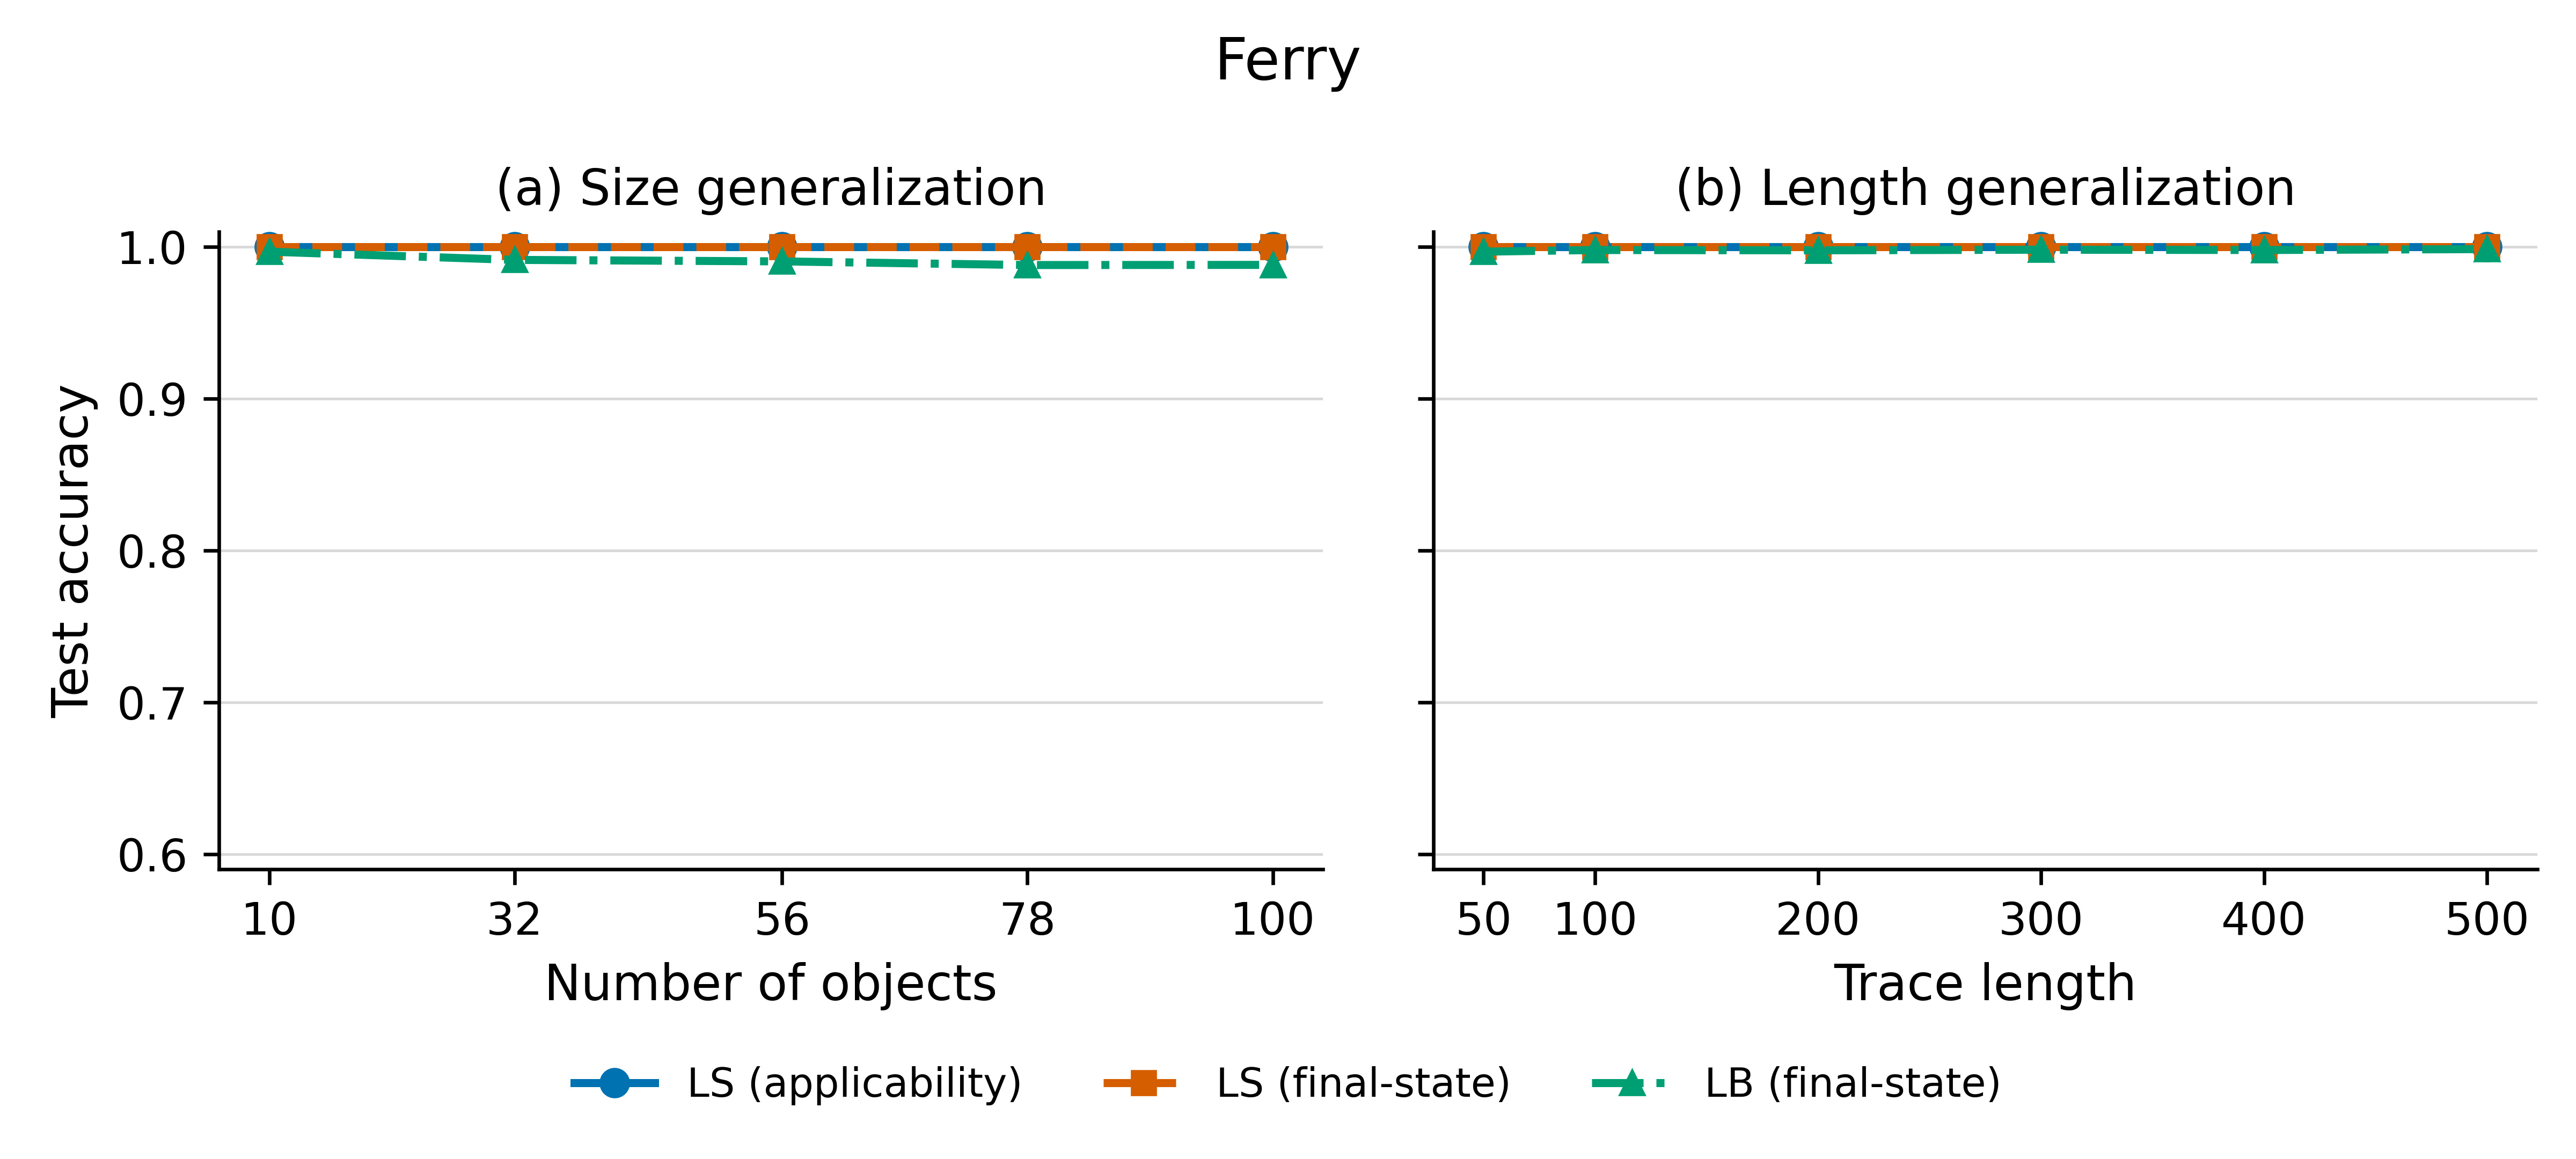
\includegraphics[width=0.85\columnwidth]{imgs/gen_plot_ferry.jpg}
    \vspace{0.2em}
    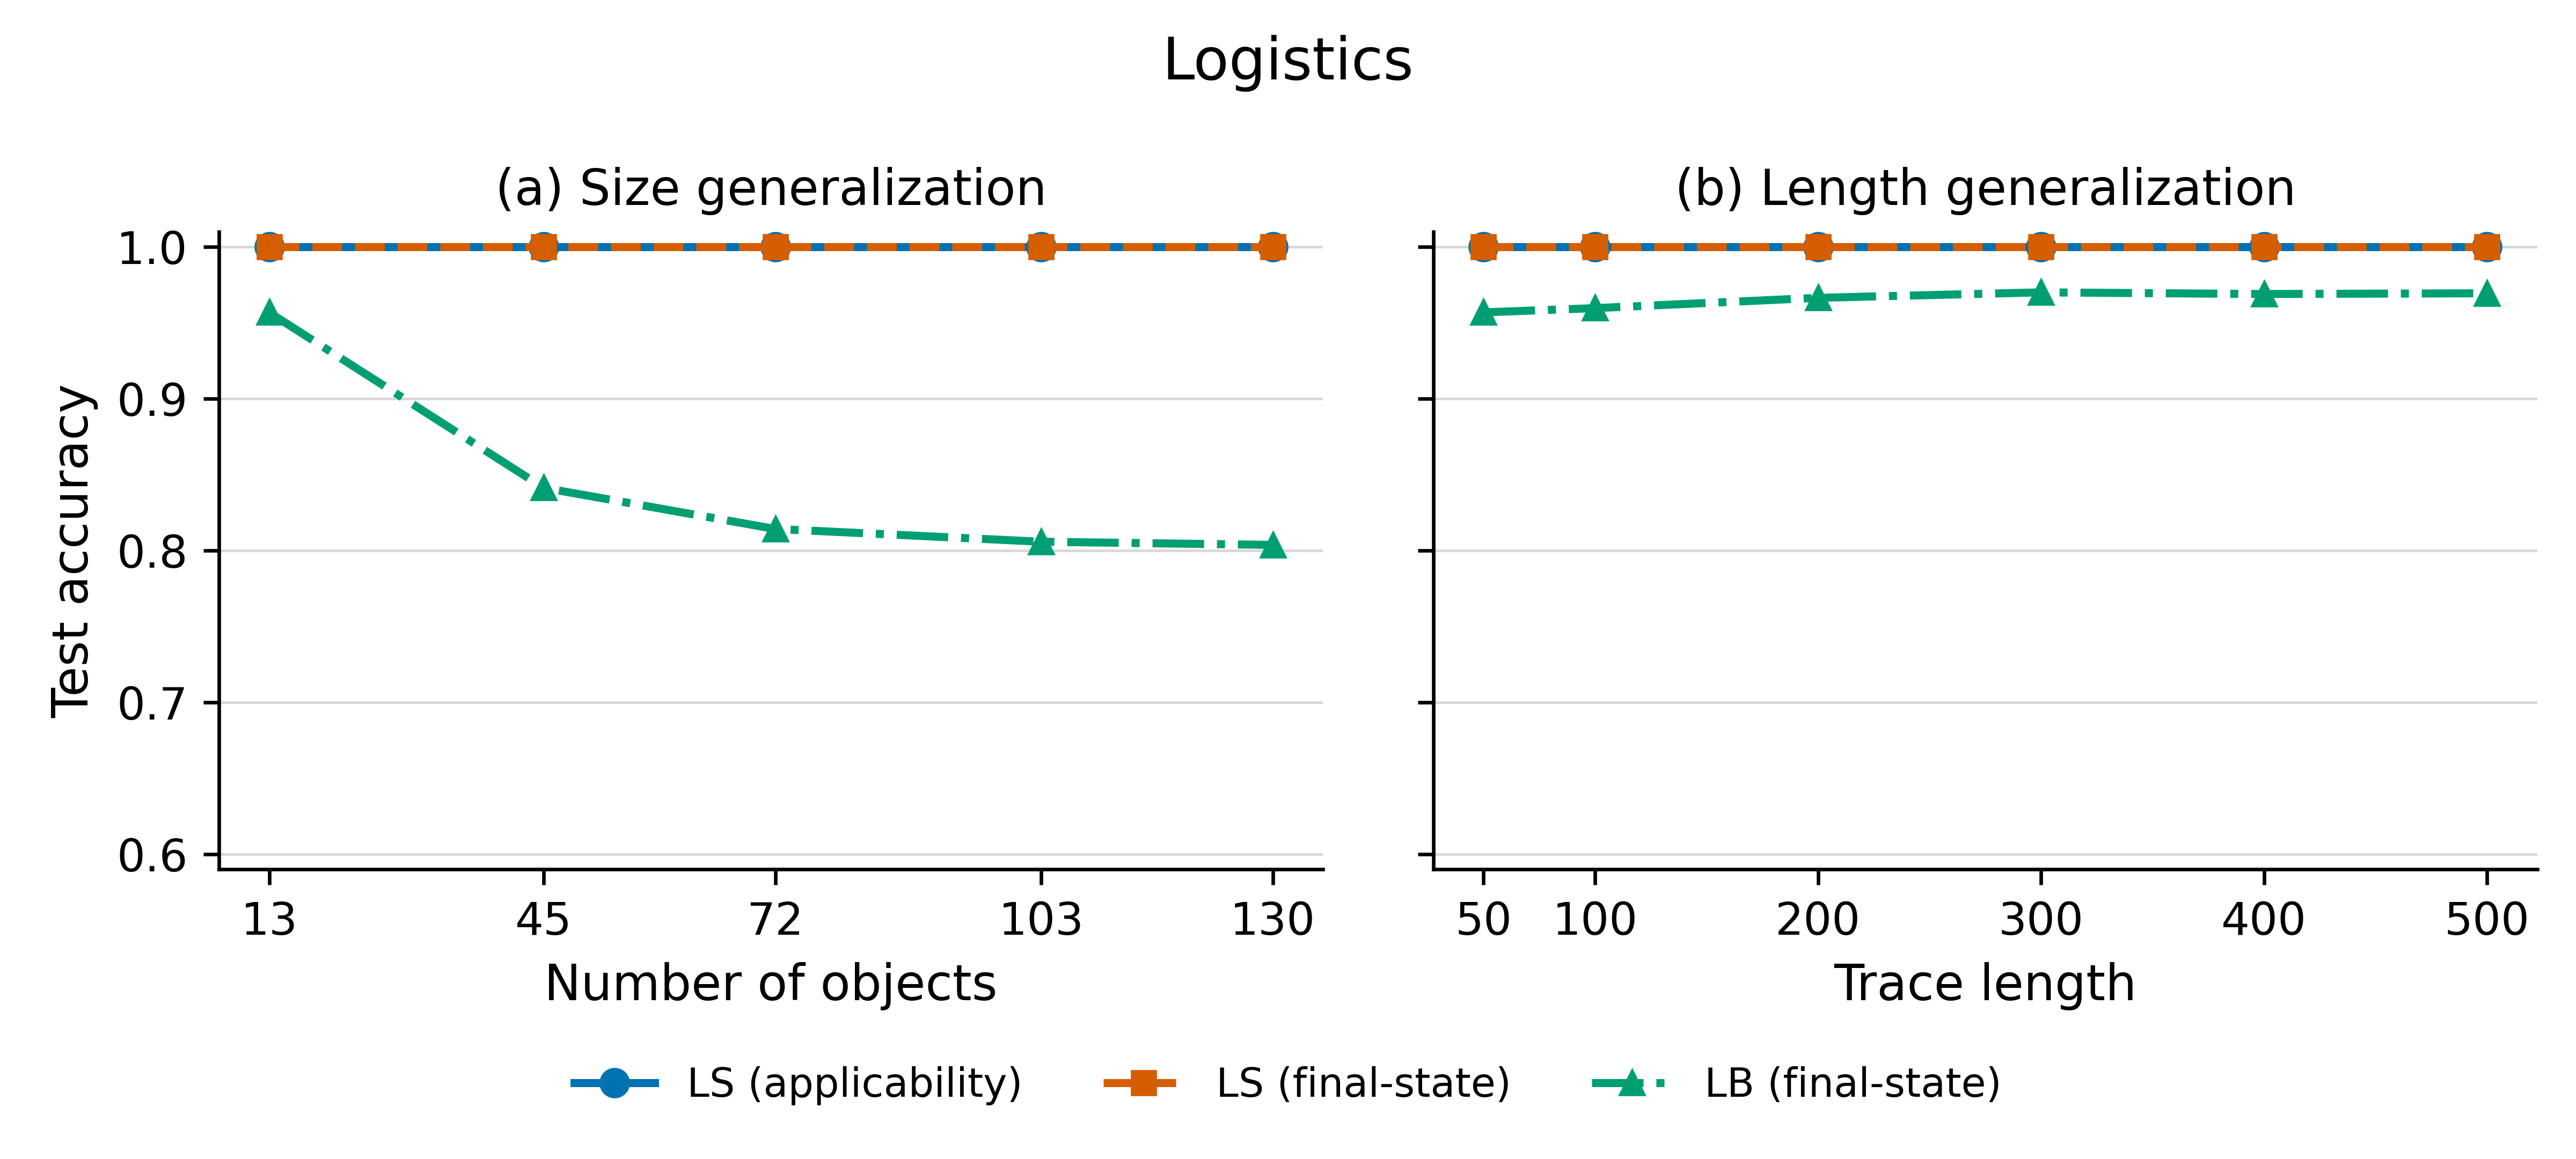
\includegraphics[width=0.85\columnwidth]{imgs/gen_plot_logistics.jpg}
    \vspace{0.2em}
    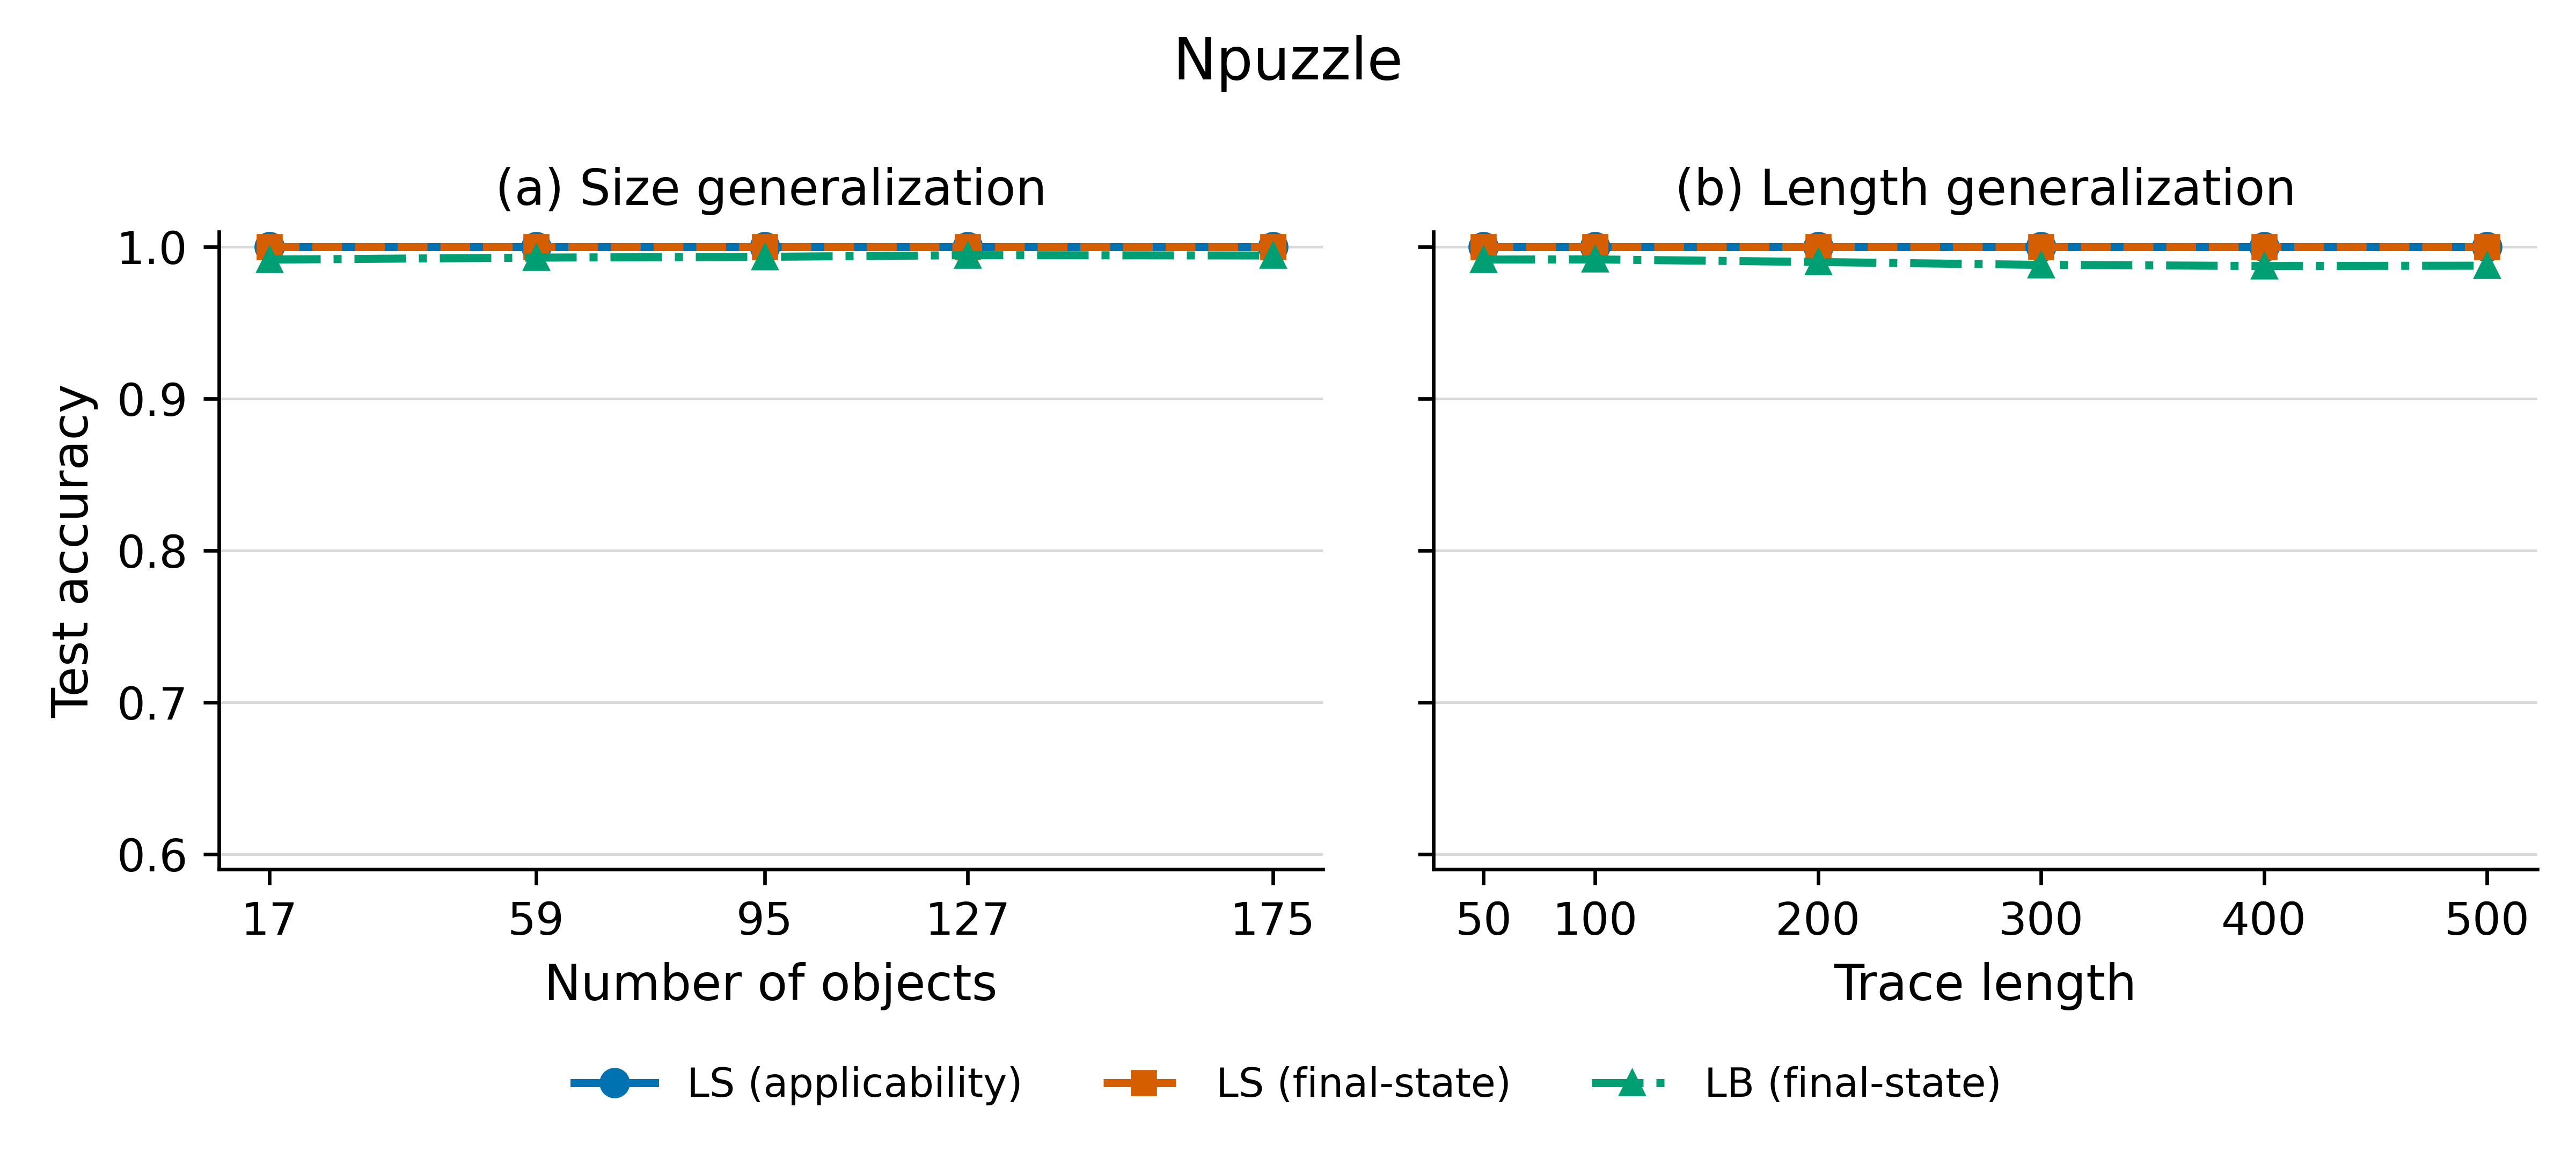
\includegraphics[width=0.85\columnwidth]{imgs/gen_plot_npuzzle.jpg}
    \vspace{0.2em}
    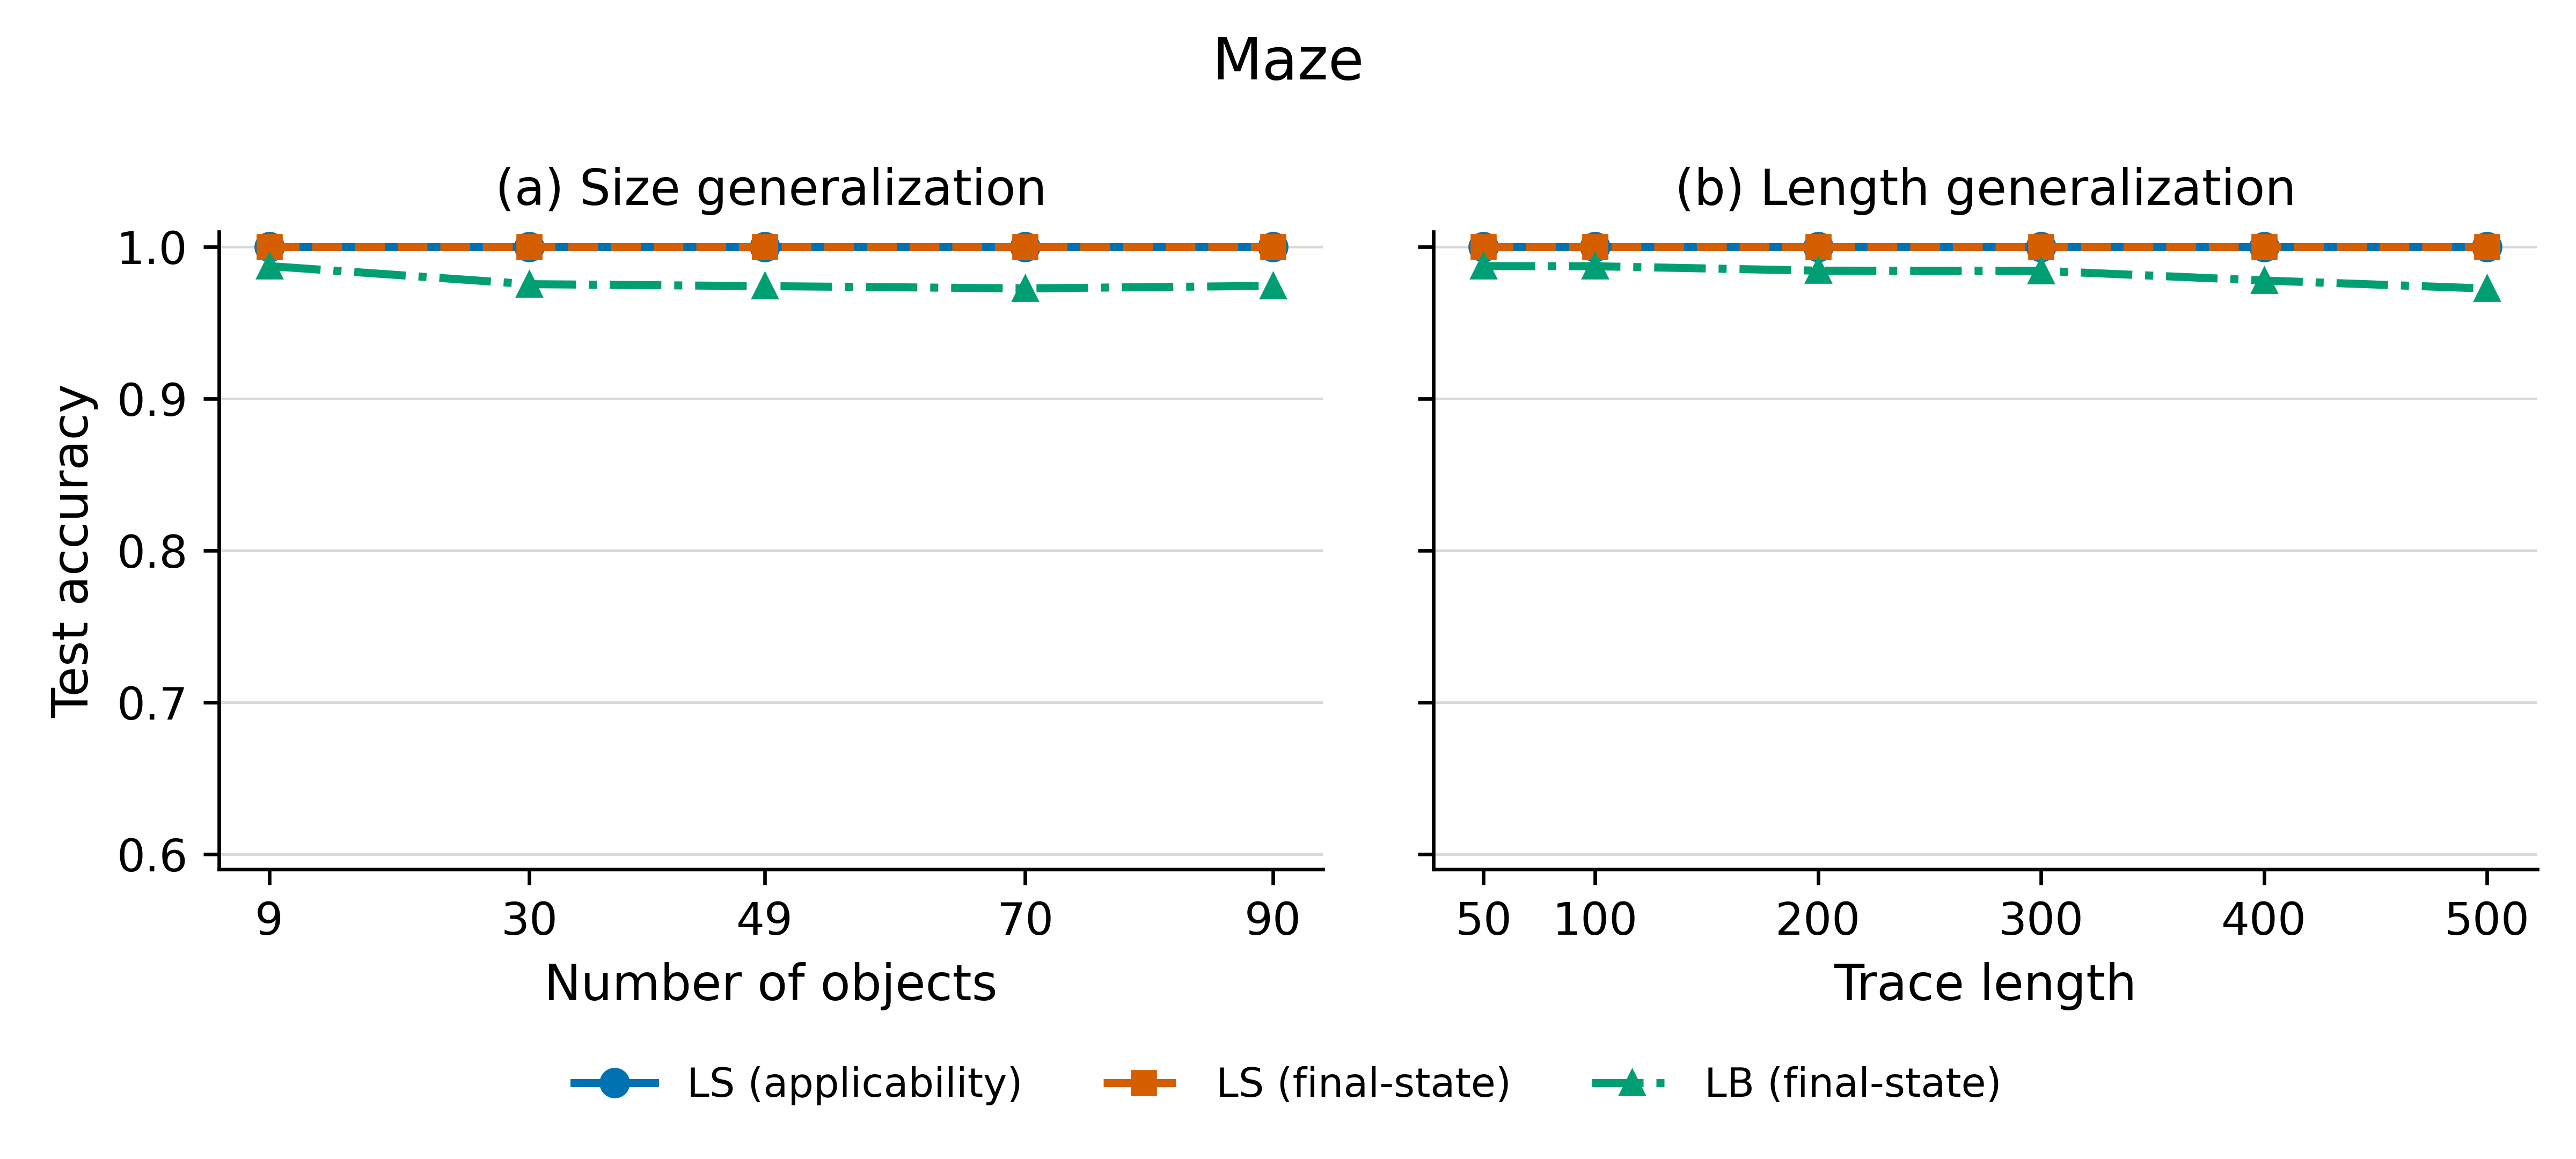
\includegraphics[width=0.85\columnwidth]{imgs/gen_plot_maze.jpg}
    \caption{\textbf{Generalization in \fr, \lgt, \mz, and \np.}
    }
    \label{fig:gen-extended}
\end{figure}


\section{Extracted \strips Models}
\label{app:strips-models}

In this section we provide the complete \strips models extracted from the LS and LB Transformers in every domain. For each transformer, we consider the seed with the best training accuracy.

\begingroup
\begin{figure*}[t]
\centering
\hrule height 0.8pt
\vspace{0.6em}
\noindent
% strips_gt_app: seed 1, training accuracy 1
\begin{minipage}[t]{0.33\textwidth}
\vspace{0pt}
{\centering (a) LS (applicability)\par}
\begin{lstlisting}
(:predicates
 (clear ?x)
 (handempty)
 (on ?x ?y)
 (ontable ?x)
 (p3 ?x))

(:action pick-up
 :parameters (?x)
 :precondition (and
  (clear ?x)
  (handempty)
  (ontable ?x))
 :effect (and
  (clear ?x)
  (ontable ?x)
  (p3 ?x)
  (not (handempty))))

(:action put-down
 :parameters (?x)
 :precondition (and
  (clear ?x)
  (ontable ?x)
  (p3 ?x))
 :effect (and
  (handempty)
  (not (p3 ?x))))

(:action stack
 :parameters (?x ?y)
 :precondition (and
  (clear ?y)
  (clear ?x)
  (ontable ?x)
  (p3 ?x))
 :effect (and
  (handempty)
  (on ?x ?y)
  (not (clear ?y))
  (not (ontable ?x))
  (not (p3 ?x))))

(:action unstack
 :parameters (?x ?y)
 :precondition (and
  (clear ?x)
  (handempty)
  (on ?x ?y))
 :effect (and
  (clear ?y)
  (clear ?x)
  (ontable ?x)
  (p3 ?x)
  (not (handempty))
  (not (on ?x ?y))))
\end{lstlisting}
\end{minipage}\hfill%
% strips_gt_state: seed 1, training accuracy 1
\begin{minipage}[t]{0.33\textwidth}
\vspace{0pt}
{\centering (a) LS (final-state)\par}
\begin{lstlisting}
(:predicates
 (clear ?x)
 (handempty)
 (on ?x ?y)
 (ontable ?x)
 (holding ?x))

(:action pick-up
 :parameters (?x)
 :precondition (and
  (clear ?x)
  (handempty)
  (ontable ?x))
 :effect (and
  (holding ?x)
  (not (handempty))
  (not (clear ?x))
  (not (ontable ?x))))

(:action put-down
 :parameters (?x)
 :precondition (and
  (holding ?x))
 :effect (and
  (handempty)
  (clear ?x)
  (ontable ?x)
  (not (holding ?x))))

(:action stack
 :parameters (?x ?y)
 :precondition (and
  (clear ?y)
  (holding ?x))
 :effect (and
  (handempty)
  (on ?x ?y)
  (clear ?x)
  (not (clear ?y))
  (not (holding ?x))))

(:action unstack
 :parameters (?x ?y)
 :precondition (and
  (clear ?x)
  (handempty)
  (on ?x ?y))
 :effect (and
  (clear ?y)
  (holding ?x)
  (not (handempty))
  (not (on ?x ?y))
  (not (clear ?x))))
\end{lstlisting}
\end{minipage}\hfill%
% sb_state: seed 4, training accuracy 0.99782
\begin{minipage}[t]{0.33\textwidth}
\vspace{0pt}
{\centering (c) LB (final-state)\par}
\begin{lstlisting}
(:predicates
 (clear ?x)
 (handempty)
 (on ?x ?y)
 (ontable ?x)
 (holding ?x))

(:action pick-up
 :parameters (?x)
 :precondition (and
  (clear ?x)
  (handempty)
  (ontable ?x))
 :effect (and
  (holding ?x)
  (not (handempty))
  (not (clear ?x))
  (not (ontable ?x))))

(:action put-down
 :parameters (?x)
 :precondition (and
  (holding ?x))
 :effect (and
  (handempty)
  (clear ?x)
  (ontable ?x)
  (not (holding ?x))))

(:action stack
 :parameters (?x ?y)
 :precondition (and
  (clear ?y)
  (holding ?x))
 :effect (and
  (handempty)
  (on ?x ?y)
  (clear ?x)
  (not (clear ?y))
  (not (holding ?x))))

(:action unstack
 :parameters (?x ?y)
 :precondition (and
  (clear ?x)
  (handempty)
  (on ?x ?y))
 :effect (and
  (clear ?y)
  (holding ?x)
  (not (handempty))
  (not (on ?x ?y))
  (not (clear ?x))))
\end{lstlisting}
\end{minipage}%
\par\vspace{0.6em}
\hrule height 0.8pt
\captionsetup{position=bottom}
\captionof{lstlisting}{\textbf{\strips models extracted in \bw.}}
\label{lst:blocksworld_full}
\end{figure*}
\endgroup

\begingroup
\begin{figure*}[t]
\centering
\hrule height 0.8pt
\vspace{0.6em}
\noindent
% strips_gt_app: seed 1, training accuracy 1
\begin{minipage}[t]{0.33\textwidth}
\vspace{0pt}
{\centering (a) LS (applicability)\par}
\begin{lstlisting}
(:predicates
 (at ?x ?y)
 (at-ferry ?x)
 (empty)
 (is_car ?x)
 (is_port ?x)
 (p4 ?x))

(:action board
 :parameters (?x ?y)
 :precondition (and
  (at ?x ?y)
  (at-ferry ?y)
  (empty)
  (is_car ?x)
  (is_port ?y))
 :effect (and
  (at ?y ?x)
  (at-ferry ?x)
  (not (at ?x ?y))
  (not (empty))
  (not (is_car ?y))))

(:action debark
 :parameters (?x ?y)
 :precondition (and
  (at-ferry ?y)
  (is_car ?x)
  (is_port ?y)
  (at-ferry ?x))
 :effect (and
  (at ?x ?y)
  (empty)
  (at ?y ?x)
  (is_car ?y)
  (not (at-ferry ?x))))

(:action sail
 :parameters (?x ?y)
 :precondition (and
  (at-ferry ?x)
  (is_port ?x)
  (is_port ?y))
 :effect (and
  (at-ferry ?y)
  (is_car ?y)
  (not (at-ferry ?x))
  (not (is_car ?x))))
\end{lstlisting}
\end{minipage}\hfill%
% strips_gt_state: seed 1, training accuracy 1
\begin{minipage}[t]{0.33\textwidth}
\vspace{0pt}
{\centering (a) LS (final-state)\par}
\begin{lstlisting}
(:predicates
 (at ?x ?y)
 (at-ferry ?x)
 (empty)
 (is_car ?x)
 (is_port ?x)
 (in ?x))

(:action board
 :parameters (?x ?y)
 :precondition (and
  (at ?x ?y)
  (at-ferry ?y)
  (empty)
  (is_car ?x)
  (is_port ?y))
 :effect (and
  (in ?x)
  (not (at ?x ?y))
  (not (empty))))

(:action debark
 :parameters (?x ?y)
 :precondition (and
  (at-ferry ?y)
  (is_car ?x)
  (is_port ?y)
  (in ?x))
 :effect (and
  (at ?x ?y)
  (empty)
  (not (in ?x))))

(:action sail
 :parameters (?x ?y)
 :precondition (and
  (at-ferry ?x)
  (is_port ?x)
  (is_port ?y))
 :effect (and
  (at-ferry ?y)
  (not (at-ferry ?x))))
\end{lstlisting}
\end{minipage}\hfill%
% sb_state: seed 4, training accuracy 0.9988
\begin{minipage}[t]{0.33\textwidth}
\vspace{0pt}
{\centering (c) LB (final-state)\par}
\begin{lstlisting}
(:predicates
 (at ?x ?y)
 (at-ferry ?x)
 (empty)
 (is_car ?x)
 (is_port ?x)
 (in ?x))

(:action board
 :parameters (?x ?y)
 :precondition (and
  (at ?x ?y)
  (at-ferry ?y)
  (empty)
  (is_car ?x)
  (is_port ?y))
 :effect (and
  (in ?x)
  (not (at ?x ?y))
  (not (empty))))

(:action debark
 :parameters (?x ?y)
 :precondition (and
  (at-ferry ?y)
  (is_car ?x)
  (is_port ?y)
  (in ?x))
 :effect (and
  (at ?x ?y)
  (empty)
  (not (in ?x))))

(:action sail
 :parameters (?x ?y)
 :precondition (and
  (at-ferry ?x)
  (is_port ?x)
  (is_port ?y))
 :effect (and
  (at-ferry ?y)
  (not (at-ferry ?x))))
\end{lstlisting}
\end{minipage}%
\par\vspace{0.6em}
\hrule height 0.8pt
\captionsetup{position=bottom}
\captionof{lstlisting}{\textbf{\strips models extracted in \fr.}}
\label{lst:ferry_full}
\end{figure*}
\endgroup

\begingroup
\begin{figure*}[t]
\centering
\hrule height 0.8pt
\vspace{0.6em}
\noindent
% strips_gt_app: seed 2, training accuracy 1
\begin{minipage}[t]{0.33\textwidth}
\vspace{0pt}
{\centering (a) LS (applicability)\par}
\begin{lstlisting}
(:predicates
 (at ?x ?y)
 (in-city ?x ?y)
 (is_airplane ?x)
 (is_airport ?x)
 (is_city ?x)
 (is_location ?x)
 (is_package ?x)
 (is_truck ?x)
 (is_vehicle ?x)
 (p9 ?x ?y))

(:action drive
 :parameters (?x ?y ?z ?u)
 :precondition (and
  (in-city ?y ?u)
  (in-city ?z ?u)
  (is_city ?u)
  (is_truck ?x)
  (is_vehicle ?x)
  (at ?x ?y))
 :effect (and
  (at ?x ?z)
  (at ?x ?u)
  (at ?y ?x)
  (at ?z ?u)
  (in-city ?x ?z)
  (in-city ?y ?u)
  (is_airplane ?y)
  (is_city ?u)
  (is_location ?z)
  (is_truck ?x)
  (not (at ?x ?y))
  (not (in-city ?x ?y))))

(:action fly
 :parameters (?x ?y ?z)
 :precondition (and
  (is_airplane ?x)
  (is_airport ?z)
  (is_location ?y)
  (is_vehicle ?x)
  (at ?x ?y))
 :effect (and
  (at ?x ?z)
  (at ?y ?x)
  (at ?y ?z)
  (at ?z ?x)
  (at ?z ?y)
  (in-city ?x ?z)
  (is_airplane ?y)
  (is_airplane ?z)
  (is_airport ?z)
  (is_location ?y)
  (is_location ?z)
  (not (at ?x ?y))))
\end{lstlisting}
\end{minipage}\hfill%
% strips_gt_state: seed 1, training accuracy 1
\begin{minipage}[t]{0.33\textwidth}
\vspace{0pt}
{\centering (a) LS (final-state)\par}
\begin{lstlisting}
(:predicates
 (at ?x ?y)
 (in-city ?x ?y)
 (is_airplane ?x)
 (is_airport ?x)
 (is_city ?x)
 (is_location ?x)
 (is_package ?x)
 (is_truck ?x)
 (is_vehicle ?x)
 (in ?x ?y))

(:action drive
 :parameters (?x ?y ?z ?u)
 :precondition (and
  (in-city ?y ?u)
  (in-city ?z ?u)
  (is_city ?u)
  (is_truck ?x)
  (is_vehicle ?x)
  (at ?x ?y)
  (is_location ?y)
  (is_location ?z))
 :effect (and
  (at ?x ?z)
  (not (at ?x ?y))))

(:action fly
 :parameters (?x ?y ?z)
 :precondition (and
  (is_airplane ?x)
  (is_airport ?z)
  (is_location ?y)
  (is_vehicle ?x)
  (at ?x ?y)
  (is_airport ?y)
  (is_location ?z))
 :effect (and
  (at ?x ?z)
  (not (at ?x ?y))))
\end{lstlisting}
\end{minipage}\hfill%
% sb_state: seed 3, training accuracy 0.97972
\begin{minipage}[t]{0.33\textwidth}
\vspace{0pt}
{\centering (c) LB (final-state)\par}
\begin{lstlisting}
(:predicates
 (at ?x ?y)
 (in-city ?x ?y)
 (is_airplane ?x)
 (is_airport ?x)
 (is_city ?x)
 (is_location ?x)
 (is_package ?x)
 (is_truck ?x)
 (is_vehicle ?x)
 (in ?x ?y))

(:action drive
 :parameters (?x ?y ?z ?u)
 :precondition (and
  (in-city ?y ?u)
  (in-city ?z ?u)
  (is_city ?u)
  (is_truck ?x)
  (is_vehicle ?x)
  (is_location ?y)
  (is_location ?z))
 :effect (and
  (at ?x ?z)
  (not (at ?x ?y))))

(:action fly
 :parameters (?x ?y ?z)
 :precondition (and
  (is_airplane ?x)
  (is_airport ?z)
  (is_location ?y)
  (is_vehicle ?x)
  (is_airport ?y)
  (is_location ?z))
 :effect (and
  (at ?x ?z)
  (not (at ?x ?y))))
\end{lstlisting}
\end{minipage}%
\par\vspace{0.6em}
\hrule height 0.8pt
\captionsetup{position=bottom}
\captionof{lstlisting}{\textbf{\strips models extracted in \lgt.}}
\label{lst:logistics_full}
\end{figure*}
\endgroup

\begingroup
\begin{figure*}[t]
\centering
\hrule height 0.8pt
\vspace{0.6em}
\noindent
% strips_gt_app: seed 2, training accuracy 1
\begin{minipage}[t]{0.33\textwidth}
\vspace{0pt}
{\centering (a) LS (applicability)\par}
\begin{lstlisting}
(:action load
 :parameters (?x ?y ?z)
 :precondition (and
  (is_location ?z)
  (is_package ?y)
  (is_vehicle ?x)
  (at ?x ?z)
  (at ?y ?z))
 :effect (and
  (at ?x ?z)
  (at ?y ?x)
  (at ?z ?x)
  (at ?z ?y)
  (in-city ?x ?y)
  (in-city ?x ?z)
  (in-city ?y ?x)
  (is_airplane ?z)
  (is_city ?x)
  (is_vehicle ?x)
  (not (at ?y ?z))
  (not (is_location ?y))))

(:action unload
 :parameters (?x ?y ?z)
 :precondition (and
  (at ?x ?z)
  (is_location ?z)
  (is_package ?y)
  (in-city ?x ?z)
  (in-city ?y ?x)
  (is_city ?x))
 :effect (and
  (at ?y ?z)
  (at ?x ?z)
  (at ?y ?x)
  (at ?z ?x)
  (at ?z ?y)
  (is_airplane ?z)
  (is_location ?z)
  (not (in-city ?y ?x))
  (not (is_location ?x))))
\end{lstlisting}
\end{minipage}\hfill%
% strips_gt_state: seed 1, training accuracy 1
\begin{minipage}[t]{0.33\textwidth}
\vspace{0pt}
{\centering (a) LS (final-state)\par}
\begin{lstlisting}
(:action load
 :parameters (?x ?y ?z)
 :precondition (and
  (is_location ?z)
  (is_package ?y)
  (is_vehicle ?x)
  (at ?x ?z)
  (at ?y ?z))
 :effect (and
  (in ?y ?x)
  (not (at ?y ?z))))

(:action unload
 :parameters (?x ?y ?z)
 :precondition (and
  (at ?x ?z)
  (is_location ?z)
  (is_package ?y)
  (in ?y ?x)
  (is_vehicle ?x))
 :effect (and
  (at ?y ?z)
  (not (in ?y ?x))))
\end{lstlisting}
\end{minipage}\hfill%
% sb_state: seed 3, training accuracy 0.97972
\begin{minipage}[t]{0.33\textwidth}
\vspace{0pt}
{\centering (c) LB (final-state)\par}
\begin{lstlisting}
(:action load
 :parameters (?x ?y ?z)
 :precondition (and
  (is_location ?z)
  (is_package ?y)
  (is_vehicle ?x))
 :effect (and
  (in ?y ?x)
  (not (at ?y ?z))))

(:action unload
 :parameters (?x ?y ?z)
 :precondition (and
  (at ?x ?z)
  (is_location ?z)
  (is_package ?y)
  (in ?y ?x)
  (is_vehicle ?x))
 :effect (and
  (at ?y ?z)
  (not (in ?y ?x))))
\end{lstlisting}
\end{minipage}%
\par\vspace{0.6em}
\hrule height 0.8pt
\captionsetup{position=bottom}
\captionof{lstlisting}{\textbf{Continuation of Listing \ref{lst:logistics_full}.}}
\label{lst:logistics_full_continuation}
\end{figure*}
\endgroup


\begingroup
\begin{figure*}[t]
\centering
\hrule height 0.8pt
\vspace{0.6em}
\noindent
% strips_gt_app: seed 1, training accuracy 1
\begin{minipage}[t]{0.33\textwidth}
\vspace{0pt}
{\centering (a) LS (applicability)\par}
\begin{lstlisting}
(:predicates
 (at ?x ?y)
 (empty ?x)
 (is_position ?x)
 (is_tile ?x)
 (neighbor ?x ?y))

(:action move
 :parameters (?x ?y ?z)
 :precondition (and
  (at ?x ?y)
  (empty ?z)
  (is_position ?y)
  (is_tile ?x)
  (neighbor ?y ?z)
  (neighbor ?z ?y))
 :effect (and
  (at ?x ?z)
  (empty ?y)
  (at ?y ?z)
  (at ?z ?y)
  (neighbor ?x ?y)
  (neighbor ?x ?z)
  (neighbor ?y ?z)
  (not (at ?x ?y))
  (not (empty ?z))
  (not (is_position ?x))))
\end{lstlisting}
\end{minipage}\hfill%
% strips_gt_state: seed 1, training accuracy 1
\begin{minipage}[t]{0.33\textwidth}
\vspace{0pt}
{\centering (a) LS (final-state)\par}
\begin{lstlisting}
(:predicates
 (at ?x ?y)
 (empty ?x)
 (is_position ?x)
 (is_tile ?x)
 (neighbor ?x ?y))

(:action move
 :parameters (?x ?y ?z)
 :precondition (and
  (at ?x ?y)
  (empty ?z)
  (is_position ?y)
  (is_tile ?x)
  (neighbor ?y ?z)
  (neighbor ?z ?y)
  (is_position ?z))
 :effect (and
  (at ?x ?z)
  (empty ?y)
  (not (at ?x ?y))
  (not (empty ?z))))
\end{lstlisting}
\end{minipage}\hfill%
% sb_state: seed 5, training accuracy 0.99175
\begin{minipage}[t]{0.33\textwidth}
\vspace{0pt}
{\centering (c) LB (final-state)\par}
\begin{lstlisting}
(:predicates
 (at ?x ?y)
 (empty ?x)
 (is_position ?x)
 (is_tile ?x)
 (neighbor ?x ?y))

(:action move
 :parameters (?x ?y ?z)
 :precondition (and
  (at ?x ?y)
  (empty ?z)
  (is_position ?y)
  (is_tile ?x)
  (neighbor ?y ?z)
  (neighbor ?z ?y)
  (is_position ?z))
 :effect (and
  (at ?x ?z)
  (empty ?y)
  (not (at ?x ?y))
  (not (empty ?z))))
\end{lstlisting}
\end{minipage}%
\par\vspace{0.6em}
\hrule height 0.8pt
\captionsetup{position=bottom}
\captionof{lstlisting}{\textbf{\strips models extracted in \np.}}
\label{lst:npuzzle_full}
\end{figure*}
\endgroup

\begingroup
\begin{figure*}[t]
\centering
\hrule height 0.8pt
\vspace{0.6em}
\noindent
% strips_gt_app: seed 1, training accuracy 1
\begin{minipage}[t]{0.33\textwidth}
\vspace{0pt}
{\centering (a) LS (applicability)\par}
\begin{lstlisting}
(:predicates
 (at ?x)
 (connected ?x ?y)
 (free ?x))

(:action move
 :parameters (?x ?y)
 :precondition (and
  (at ?x)
  (connected ?x ?y)
  (connected ?y ?x)
  (free ?x)
  (free ?y))
 :effect (and
  (at ?y)
  (not (at ?x))))
\end{lstlisting}
\end{minipage}\hfill%
% strips_gt_state: seed 1, training accuracy 1
\begin{minipage}[t]{0.33\textwidth}
\vspace{0pt}
{\centering (a) LS (final-state)\par}
\begin{lstlisting}
(:predicates
 (at ?x)
 (connected ?x ?y)
 (free ?x))

(:action move
 :parameters (?x ?y)
 :precondition (and
  (at ?x)
  (connected ?x ?y)
  (connected ?y ?x)
  (free ?x)
  (free ?y))
 :effect (and
  (at ?y)
  (not (at ?x))))
\end{lstlisting}
\end{minipage}\hfill%
% sb_state: seed 5, training accuracy 0.98856
\begin{minipage}[t]{0.33\textwidth}
\vspace{0pt}
{\centering (c) LB (final-state)\par}
\begin{lstlisting}
(:predicates
 (at ?x)
 (connected ?x ?y)
 (free ?x))

(:action move
 :parameters (?x ?y)
 :precondition (and
  (at ?x)
  (connected ?x ?y)
  (connected ?y ?x)
  (free ?x)
  (free ?y))
 :effect (and
  (at ?y)
  (not (at ?x))))
\end{lstlisting}
\end{minipage}%
\par\vspace{0.6em}
\hrule height 0.8pt
\captionsetup{position=bottom}
\captionof{lstlisting}{\textbf{\strips models extracted in \mz.}}
\label{lst:mazefree_full}
\end{figure*}
\endgroup


\end{document}




\iffalse
    
    Given an unknown \strips model
    $M=\langle\mathcal{P},A\rangle$ and a set $T$ of traces drawn from
    problem instances $P=\langle M,O_N,I,G\rangle$, the learning task is to
    recover $M$ from $T$. Each trace contains an initial state $I$ and a sequence
    $\tau=(a_0,\ldots,a_{n-1})$ of ground actions obtained by instantiating the
    action schemas in $A$ with objects from $O_N$. The goal $G$ of the
    corresponding instance is not used for learning.
    
    We encode the initial state $I$ at the beginning of each trace, allowing
    traces to be drawn from different problem instances where action
    applicability may depend on facts that cannot be inferred from the preceding
    actions alone.
    
    Given $I$ and an action sequence $\tau$, let
    $$
    f_M(I,\tau)=
    \begin{cases}
    0, & \text{if $\tau$ is applicable from $I$ according to $M$},\\
    1, & \text{otherwise}.
    \end{cases}
    $$
    From the perspective of next-token prediction, an action $a$ is a possible
    next action after an applicable prefix $\tau$ precisely when
    $f_M(I,\langle\tau,a\rangle)=0$.
    
    A Transformer can provide a parametrized, differentiable approximation
    $f_\theta(I,\tau)\in[0,1]$ to this Boolean function, with parameters $\theta$
    optimized so that $f_\theta$ agrees with $f_M$ on the observed traces and
    generalizes to unseen traces and problem instances.
    
    For a fixed finite object set and fixed $\theta$, $f_\theta$ defines a
    recognizer over encoded initial-state and action-trace pairs. Learning then
    amounts to finding parameters for which the recognized language matches that
    induced by $M$. This connects the task to masked hard-attention Transformers,
    \brasp, and the formal language of valid \strips
    traces~\citep{yang2024masked,Lin_Bercher_2022}, motivating our first setting,
    \emph{applicability supervision}. Here, traces contain applicable and
    inapplicable actions with their labels, but no states after the initial one.
    
    Alternatively, we can train only on applicable action sequences and use
    their resulting final states as supervision. This yields
    \emph{final-state supervision}, where each trace contains an initial state,
    an applicable action sequence, and its final state, while intermediate states
    remain unobserved.
    
    \subsection{Applicability Supervision} 
\fi